\documentclass[twoside]{book}

% Packages required by doxygen
\usepackage{fixltx2e}
\usepackage{calc}
\usepackage{doxygen}
\usepackage[export]{adjustbox} % also loads graphicx
\usepackage{graphicx}
\usepackage[utf8]{inputenc}
\usepackage{makeidx}
\usepackage{multicol}
\usepackage{multirow}
\PassOptionsToPackage{warn}{textcomp}
\usepackage{textcomp}
\usepackage[nointegrals]{wasysym}
\usepackage[table]{xcolor}

% Font selection
\usepackage[T1]{fontenc}
\usepackage[scaled=.90]{helvet}
\usepackage{courier}
\usepackage{amssymb}
\usepackage{sectsty}
\renewcommand{\familydefault}{\sfdefault}
\allsectionsfont{%
  \fontseries{bc}\selectfont%
  \color{darkgray}%
}
\renewcommand{\DoxyLabelFont}{%
  \fontseries{bc}\selectfont%
  \color{darkgray}%
}
\newcommand{\+}{\discretionary{\mbox{\scriptsize$\hookleftarrow$}}{}{}}

% Page & text layout
\usepackage{geometry}
\geometry{%
  a4paper,%
  top=2.5cm,%
  bottom=2.5cm,%
  left=2.5cm,%
  right=2.5cm%
}
\tolerance=750
\hfuzz=15pt
\hbadness=750
\setlength{\emergencystretch}{15pt}
\setlength{\parindent}{0cm}
\setlength{\parskip}{3ex plus 2ex minus 2ex}
\makeatletter
\renewcommand{\paragraph}{%
  \@startsection{paragraph}{4}{0ex}{-1.0ex}{1.0ex}{%
    \normalfont\normalsize\bfseries\SS@parafont%
  }%
}
\renewcommand{\subparagraph}{%
  \@startsection{subparagraph}{5}{0ex}{-1.0ex}{1.0ex}{%
    \normalfont\normalsize\bfseries\SS@subparafont%
  }%
}
\makeatother

% Headers & footers
\usepackage{fancyhdr}
\pagestyle{fancyplain}
\fancyhead[LE]{\fancyplain{}{\bfseries\thepage}}
\fancyhead[CE]{\fancyplain{}{}}
\fancyhead[RE]{\fancyplain{}{\bfseries\leftmark}}
\fancyhead[LO]{\fancyplain{}{\bfseries\rightmark}}
\fancyhead[CO]{\fancyplain{}{}}
\fancyhead[RO]{\fancyplain{}{\bfseries\thepage}}
\fancyfoot[LE]{\fancyplain{}{}}
\fancyfoot[CE]{\fancyplain{}{}}
\fancyfoot[RE]{\fancyplain{}{\bfseries\scriptsize Generated by Doxygen }}
\fancyfoot[LO]{\fancyplain{}{\bfseries\scriptsize Generated by Doxygen }}
\fancyfoot[CO]{\fancyplain{}{}}
\fancyfoot[RO]{\fancyplain{}{}}
\renewcommand{\footrulewidth}{0.4pt}
\renewcommand{\chaptermark}[1]{%
  \markboth{#1}{}%
}
\renewcommand{\sectionmark}[1]{%
  \markright{\thesection\ #1}%
}

% Indices & bibliography
\usepackage{natbib}
\usepackage[titles]{tocloft}
\setcounter{tocdepth}{3}
\setcounter{secnumdepth}{5}
\makeindex

% Hyperlinks (required, but should be loaded last)
\usepackage{ifpdf}
\ifpdf
  \usepackage[pdftex,pagebackref=true]{hyperref}
\else
  \usepackage[ps2pdf,pagebackref=true]{hyperref}
\fi
\hypersetup{%
  colorlinks=true,%
  linkcolor=blue,%
  citecolor=blue,%
  unicode%
}

% Custom commands
\newcommand{\clearemptydoublepage}{%
  \newpage{\pagestyle{empty}\cleardoublepage}%
}

\usepackage{caption}
\captionsetup{labelsep=space,justification=centering,font={bf},singlelinecheck=off,skip=4pt,position=top}

%===== C O N T E N T S =====

\begin{document}

% Titlepage & ToC
\hypersetup{pageanchor=false,
             bookmarksnumbered=true,
             pdfencoding=unicode
            }
\pagenumbering{roman}
\begin{titlepage}
\vspace*{7cm}
\begin{center}%
{\Large Crosmi \\[1ex]\large 1.\+0 }\\
\vspace*{1cm}
{\large Generated by Doxygen 1.8.11}\\
\end{center}
\end{titlepage}
\clearemptydoublepage
\tableofcontents
\clearemptydoublepage
\pagenumbering{arabic}
\hypersetup{pageanchor=true}

%--- Begin generated contents ---
\chapter{Data Structure Index}
\section{Data Structures}
Here are the data structures with brief descriptions\+:\begin{DoxyCompactList}
\item\contentsline{section}{\hyperlink{struct_buffer}{Buffer} }{\pageref{struct_buffer}}{}
\end{DoxyCompactList}

\chapter{File Index}
\section{File List}
Here is a list of all files with brief descriptions\+:\begin{DoxyCompactList}
\item\contentsline{section}{\hyperlink{main_8c}{main.\+c} }{\pageref{main_8c}}{}
\item\contentsline{section}{\hyperlink{our_a_d_c_8c}{our\+A\+D\+C.\+c} }{\pageref{our_a_d_c_8c}}{}
\item\contentsline{section}{\hyperlink{our_a_d_c_8h}{our\+A\+D\+C.\+h} }{\pageref{our_a_d_c_8h}}{}
\item\contentsline{section}{\hyperlink{our_d_a_c_8c}{our\+D\+A\+C.\+c} }{\pageref{our_d_a_c_8c}}{}
\item\contentsline{section}{\hyperlink{our_d_a_c_8h}{our\+D\+A\+C.\+h} }{\pageref{our_d_a_c_8h}}{}
\item\contentsline{section}{\hyperlink{our_d_m_a_8c}{our\+D\+M\+A.\+c} }{\pageref{our_d_m_a_8c}}{}
\item\contentsline{section}{\hyperlink{our_d_m_a_8h}{our\+D\+M\+A.\+h} }{\pageref{our_d_m_a_8h}}{}
\item\contentsline{section}{\hyperlink{our_pintza_8c}{our\+Pintza.\+c} }{\pageref{our_pintza_8c}}{}
\item\contentsline{section}{\hyperlink{our_pintza_8h}{our\+Pintza.\+h} }{\pageref{our_pintza_8h}}{}
\item\contentsline{section}{\hyperlink{our_rcc_gpio_8c}{our\+Rcc\+Gpio.\+c} }{\pageref{our_rcc_gpio_8c}}{}
\item\contentsline{section}{\hyperlink{our_rcc_gpio_8h}{our\+Rcc\+Gpio.\+h} }{\pageref{our_rcc_gpio_8h}}{}
\item\contentsline{section}{\hyperlink{our_systick_8c}{our\+Systick.\+c} }{\pageref{our_systick_8c}}{}
\item\contentsline{section}{\hyperlink{our_systick_8h}{our\+Systick.\+h} }{\pageref{our_systick_8h}}{}
\item\contentsline{section}{\hyperlink{our_timer_8c}{our\+Timer.\+c} }{\pageref{our_timer_8c}}{}
\item\contentsline{section}{\hyperlink{our_timer_8h}{our\+Timer.\+h} }{\pageref{our_timer_8h}}{}
\item\contentsline{section}{\hyperlink{our_usart_8c}{our\+Usart.\+c} }{\pageref{our_usart_8c}}{}
\item\contentsline{section}{\hyperlink{our_usart_8h}{our\+Usart.\+h} }{\pageref{our_usart_8h}}{}
\end{DoxyCompactList}

\chapter{Data Structure Documentation}
\hypertarget{struct_buffer}{}\section{Buffer Struct Reference}
\label{struct_buffer}\index{Buffer@{Buffer}}
\subsection*{Data Fields}
\begin{DoxyCompactItemize}
\item 
uint32\+\_\+t \hyperlink{struct_buffer_ab2c6b258f02add8fdf4cfc7c371dd772}{size}
\item 
uint8\+\_\+t \hyperlink{struct_buffer_a97eaba5b61706891a4da114bde40da4d}{buffer} \mbox{[}\hyperlink{our_usart_8c_a6b20d41d6252e9871430c242cb1a56e7}{B\+U\+F\+F\+E\+R\+\_\+\+S\+I\+ZE}\mbox{]}
\end{DoxyCompactItemize}


\subsection{Field Documentation}
\index{Buffer@{Buffer}!buffer@{buffer}}
\index{buffer@{buffer}!Buffer@{Buffer}}
\subsubsection[{\texorpdfstring{buffer}{buffer}}]{\setlength{\rightskip}{0pt plus 5cm}uint8\+\_\+t buffer\mbox{[}{\bf B\+U\+F\+F\+E\+R\+\_\+\+S\+I\+ZE}\mbox{]}}\hypertarget{struct_buffer_a97eaba5b61706891a4da114bde40da4d}{}\label{struct_buffer_a97eaba5b61706891a4da114bde40da4d}
\index{Buffer@{Buffer}!size@{size}}
\index{size@{size}!Buffer@{Buffer}}
\subsubsection[{\texorpdfstring{size}{size}}]{\setlength{\rightskip}{0pt plus 5cm}uint32\+\_\+t size}\hypertarget{struct_buffer_ab2c6b258f02add8fdf4cfc7c371dd772}{}\label{struct_buffer_ab2c6b258f02add8fdf4cfc7c371dd772}


The documentation for this struct was generated from the following file\+:\begin{DoxyCompactItemize}
\item 
\hyperlink{our_usart_8c}{our\+Usart.\+c}\end{DoxyCompactItemize}

\chapter{File Documentation}
\hypertarget{main_8c}{}\section{main.\+c File Reference}
\label{main_8c}\index{main.\+c@{main.\+c}}
{\ttfamily \#include \char`\"{}our\+Usart.\+h\char`\"{}}\\*
{\ttfamily \#include \char`\"{}our\+Pintza.\+h\char`\"{}}\\*
{\ttfamily \#include \char`\"{}our\+Rcc\+Gpio.\+h\char`\"{}}\\*
{\ttfamily \#include \char`\"{}our\+Systick.\+h\char`\"{}}\\*
Include dependency graph for main.\+c\+:
\nopagebreak
\begin{figure}[H]
\begin{center}
\leavevmode
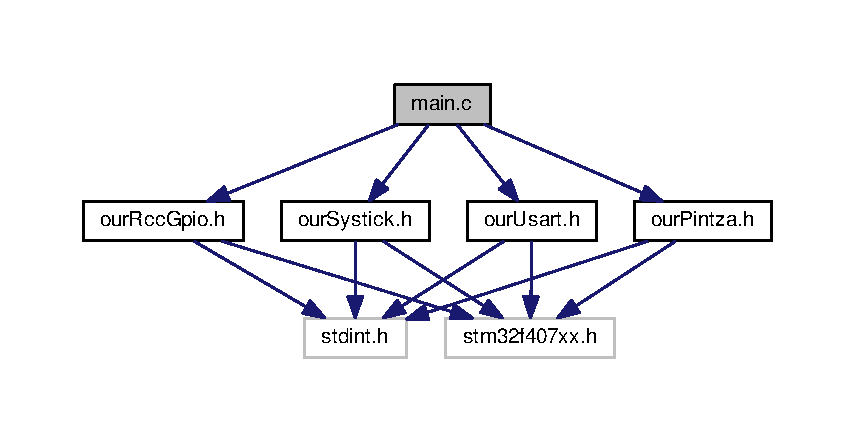
\includegraphics[width=350pt]{main_8c__incl}
\end{center}
\end{figure}
\subsection*{Functions}
\begin{DoxyCompactItemize}
\item 
void \hyperlink{main_8c_a2821d444d59e2408901a458e209a403d}{irakurri} (void)
\item 
void \hyperlink{main_8c_ad442c62b85591b16bbebcc35c9e63dc3}{init\+G\+P\+IO} (void)
\item 
int \hyperlink{main_8c_ae66f6b31b5ad750f1fe042a706a4e3d4}{main} ()
\end{DoxyCompactItemize}
\subsection*{Variables}
\begin{DoxyCompactItemize}
\item 
uint32\+\_\+t \hyperlink{main_8c_a16a718662c2078f4000abfce9a61dbc2}{piztuta} = 1
\end{DoxyCompactItemize}


\subsection{Function Documentation}
\index{main.\+c@{main.\+c}!init\+G\+P\+IO@{init\+G\+P\+IO}}
\index{init\+G\+P\+IO@{init\+G\+P\+IO}!main.\+c@{main.\+c}}
\subsubsection[{\texorpdfstring{init\+G\+P\+I\+O(void)}{initGPIO(void)}}]{\setlength{\rightskip}{0pt plus 5cm}void init\+G\+P\+IO (
\begin{DoxyParamCaption}
\item[{void}]{}
\end{DoxyParamCaption}
)}\hypertarget{main_8c_ad442c62b85591b16bbebcc35c9e63dc3}{}\label{main_8c_ad442c62b85591b16bbebcc35c9e63dc3}
\index{main.\+c@{main.\+c}!irakurri@{irakurri}}
\index{irakurri@{irakurri}!main.\+c@{main.\+c}}
\subsubsection[{\texorpdfstring{irakurri(void)}{irakurri(void)}}]{\setlength{\rightskip}{0pt plus 5cm}void irakurri (
\begin{DoxyParamCaption}
\item[{void}]{}
\end{DoxyParamCaption}
)}\hypertarget{main_8c_a2821d444d59e2408901a458e209a403d}{}\label{main_8c_a2821d444d59e2408901a458e209a403d}
\index{main.\+c@{main.\+c}!main@{main}}
\index{main@{main}!main.\+c@{main.\+c}}
\subsubsection[{\texorpdfstring{main()}{main()}}]{\setlength{\rightskip}{0pt plus 5cm}int main (
\begin{DoxyParamCaption}
{}
\end{DoxyParamCaption}
)}\hypertarget{main_8c_ae66f6b31b5ad750f1fe042a706a4e3d4}{}\label{main_8c_ae66f6b31b5ad750f1fe042a706a4e3d4}


\subsection{Variable Documentation}
\index{main.\+c@{main.\+c}!piztuta@{piztuta}}
\index{piztuta@{piztuta}!main.\+c@{main.\+c}}
\subsubsection[{\texorpdfstring{piztuta}{piztuta}}]{\setlength{\rightskip}{0pt plus 5cm}uint32\+\_\+t piztuta = 1}\hypertarget{main_8c_a16a718662c2078f4000abfce9a61dbc2}{}\label{main_8c_a16a718662c2078f4000abfce9a61dbc2}

\hypertarget{our_a_d_c_8c}{}\section{our\+A\+D\+C.\+c File Reference}
\label{our_a_d_c_8c}\index{our\+A\+D\+C.\+c@{our\+A\+D\+C.\+c}}
{\ttfamily \#include \char`\"{}our\+A\+D\+C.\+h\char`\"{}}\\*
Include dependency graph for our\+A\+D\+C.\+c\+:
\nopagebreak
\begin{figure}[H]
\begin{center}
\leavevmode
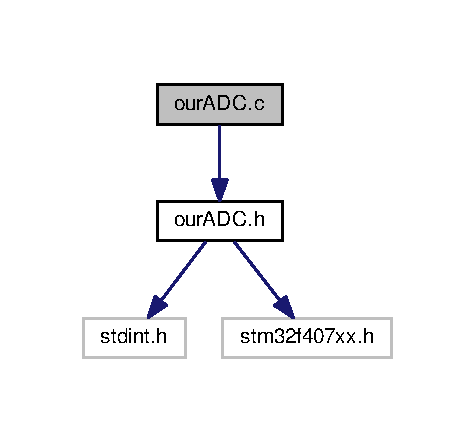
\includegraphics[width=228pt]{our_a_d_c_8c__incl}
\end{center}
\end{figure}
\subsection*{Functions}
\begin{DoxyCompactItemize}
\item 
void \hyperlink{our_a_d_c_8c_a717656252b7f23c44aee8c93d8781965}{init\+A\+DC} (uint32\+\_\+t timer2\+T\+R\+GO, uint32\+\_\+t interrupzioa, uint32\+\_\+t kanala)
\item 
void \hyperlink{our_a_d_c_8c_a21c5d304a223b06f835851d581cbd697}{switch\+A\+DC} (int piztu)
\item 
void \hyperlink{our_a_d_c_8c_a443125cba6c904aa284362d5ff18d459}{set\+A\+D\+C\+Call\+Back} (void($\ast$funtzioa)(uint16\+\_\+t))
\item 
void \hyperlink{our_a_d_c_8c_a5438868d5b3d3b592e5ad99f04aa1735}{our\+A\+D\+C\+Handler} ()
\item 
uint16\+\_\+t \hyperlink{our_a_d_c_8c_a66772f4f6e5904d8a80a446857d59e39}{get\+Azken\+Balioa} ()
\item 
uint16\+\_\+t \hyperlink{our_a_d_c_8c_a38923b0842879b8f18e204a2cec0e67a}{get\+Balioa} (void)
\end{DoxyCompactItemize}
\subsection*{Variables}
\begin{DoxyCompactItemize}
\item 
uint16\+\_\+t \hyperlink{our_a_d_c_8c_a7a8a779a9dee44110b8999ab941d2a33}{azken\+Balioa} = 0
\item 
void($\ast$ \hyperlink{our_a_d_c_8c_a6044b37b20956fcf3b5c86e72ba091e5}{callback} )(uint16\+\_\+t)=0
\end{DoxyCompactItemize}


\subsection{Function Documentation}
\index{our\+A\+D\+C.\+c@{our\+A\+D\+C.\+c}!get\+Azken\+Balioa@{get\+Azken\+Balioa}}
\index{get\+Azken\+Balioa@{get\+Azken\+Balioa}!our\+A\+D\+C.\+c@{our\+A\+D\+C.\+c}}
\subsubsection[{\texorpdfstring{get\+Azken\+Balioa()}{getAzkenBalioa()}}]{\setlength{\rightskip}{0pt plus 5cm}uint16\+\_\+t get\+Azken\+Balioa (
\begin{DoxyParamCaption}
\item[{void}]{}
\end{DoxyParamCaption}
)}\hypertarget{our_a_d_c_8c_a66772f4f6e5904d8a80a446857d59e39}{}\label{our_a_d_c_8c_a66772f4f6e5904d8a80a446857d59e39}
Function that returns the last value of A\+DC. \begin{DoxyReturn}{Returns}
azken\+Balioa\+: uint16\+\_\+t type A\+DC last value. 
\end{DoxyReturn}
\index{our\+A\+D\+C.\+c@{our\+A\+D\+C.\+c}!get\+Balioa@{get\+Balioa}}
\index{get\+Balioa@{get\+Balioa}!our\+A\+D\+C.\+c@{our\+A\+D\+C.\+c}}
\subsubsection[{\texorpdfstring{get\+Balioa(void)}{getBalioa(void)}}]{\setlength{\rightskip}{0pt plus 5cm}uint16\+\_\+t get\+Balioa (
\begin{DoxyParamCaption}
\item[{void}]{}
\end{DoxyParamCaption}
)}\hypertarget{our_a_d_c_8c_a38923b0842879b8f18e204a2cec0e67a}{}\label{our_a_d_c_8c_a38923b0842879b8f18e204a2cec0e67a}
This function return the last value. \begin{DoxyReturn}{Returns}
azken\+Balioa\+: uint16\+\_\+t type conversion\textquotesingle{}s last value. 
\end{DoxyReturn}
\index{our\+A\+D\+C.\+c@{our\+A\+D\+C.\+c}!init\+A\+DC@{init\+A\+DC}}
\index{init\+A\+DC@{init\+A\+DC}!our\+A\+D\+C.\+c@{our\+A\+D\+C.\+c}}
\subsubsection[{\texorpdfstring{init\+A\+D\+C(uint32\+\_\+t timer2\+T\+R\+G\+O, uint32\+\_\+t interrupzioa, uint32\+\_\+t kanala)}{initADC(uint32_t timer2TRGO, uint32_t interrupzioa, uint32_t kanala)}}]{\setlength{\rightskip}{0pt plus 5cm}void init\+A\+DC (
\begin{DoxyParamCaption}
\item[{uint32\+\_\+t}]{timer2\+T\+R\+GO, }
\item[{uint32\+\_\+t}]{interrupzioa, }
\item[{uint32\+\_\+t}]{kanala}
\end{DoxyParamCaption}
)}\hypertarget{our_a_d_c_8c_a717656252b7f23c44aee8c93d8781965}{}\label{our_a_d_c_8c_a717656252b7f23c44aee8c93d8781965}
This function initializes A\+DC, setting core basic params to launch A\+DC. Some of the params are optional configurations such as interruption and T\+R\+GO. 
\begin{DoxyParams}{Parameters}
{\em timer2\+T\+R\+GO} & uint32\+\_\+t type but acts as a boolean to know if timer 2\textquotesingle{}s T\+R\+GO is needed. \\
\hline
{\em interrupzioa} & uint32\+\_\+t type but acts as boolean to know if interruption is needed. \\
\hline
{\em kanala} & uint32\+\_\+t type holds the value of which channel should be used by the A\+DC. \\
\hline
\end{DoxyParams}
\begin{DoxyReturn}{Returns}
void. 
\end{DoxyReturn}
\index{our\+A\+D\+C.\+c@{our\+A\+D\+C.\+c}!our\+A\+D\+C\+Handler@{our\+A\+D\+C\+Handler}}
\index{our\+A\+D\+C\+Handler@{our\+A\+D\+C\+Handler}!our\+A\+D\+C.\+c@{our\+A\+D\+C.\+c}}
\subsubsection[{\texorpdfstring{our\+A\+D\+C\+Handler()}{ourADCHandler()}}]{\setlength{\rightskip}{0pt plus 5cm}void our\+A\+D\+C\+Handler (
\begin{DoxyParamCaption}
\item[{void}]{}
\end{DoxyParamCaption}
)}\hypertarget{our_a_d_c_8c_a5438868d5b3d3b592e5ad99f04aa1735}{}\label{our_a_d_c_8c_a5438868d5b3d3b592e5ad99f04aa1735}
This function acts as a handler for the interruption caused by the A\+DC. \begin{DoxyReturn}{Returns}
void. 
\end{DoxyReturn}
\index{our\+A\+D\+C.\+c@{our\+A\+D\+C.\+c}!set\+A\+D\+C\+Call\+Back@{set\+A\+D\+C\+Call\+Back}}
\index{set\+A\+D\+C\+Call\+Back@{set\+A\+D\+C\+Call\+Back}!our\+A\+D\+C.\+c@{our\+A\+D\+C.\+c}}
\subsubsection[{\texorpdfstring{set\+A\+D\+C\+Call\+Back(void($\ast$funtzioa)(uint16\+\_\+t))}{setADCCallBack(void(*funtzioa)(uint16_t))}}]{\setlength{\rightskip}{0pt plus 5cm}void set\+A\+D\+C\+Call\+Back (
\begin{DoxyParamCaption}
\item[{void($\ast$)(uint16\+\_\+t)}]{funtzioa}
\end{DoxyParamCaption}
)}\hypertarget{our_a_d_c_8c_a443125cba6c904aa284362d5ff18d459}{}\label{our_a_d_c_8c_a443125cba6c904aa284362d5ff18d459}
This function sets a pointer to another function which accepts a paramater of type uint16\+\_\+t. Callback funtcion.  funtzio\+: void type points to a function. \begin{DoxyReturn}{Returns}
void 
\end{DoxyReturn}
\index{our\+A\+D\+C.\+c@{our\+A\+D\+C.\+c}!switch\+A\+DC@{switch\+A\+DC}}
\index{switch\+A\+DC@{switch\+A\+DC}!our\+A\+D\+C.\+c@{our\+A\+D\+C.\+c}}
\subsubsection[{\texorpdfstring{switch\+A\+D\+C(int piztu)}{switchADC(int piztu)}}]{\setlength{\rightskip}{0pt plus 5cm}void switch\+A\+DC (
\begin{DoxyParamCaption}
\item[{int}]{piztu}
\end{DoxyParamCaption}
)}\hypertarget{our_a_d_c_8c_a21c5d304a223b06f835851d581cbd697}{}\label{our_a_d_c_8c_a21c5d304a223b06f835851d581cbd697}
This function enable or disable A\+DC peripheral depending on the given parameter that acts as a boolean type. 
\begin{DoxyParams}{Parameters}
{\em piztu} & int type but acts as a boolean to know whether is needed to enable or disable A\+D\+C1. \\
\hline
\end{DoxyParams}
\begin{DoxyReturn}{Returns}
void. 
\end{DoxyReturn}


\subsection{Variable Documentation}
\index{our\+A\+D\+C.\+c@{our\+A\+D\+C.\+c}!azken\+Balioa@{azken\+Balioa}}
\index{azken\+Balioa@{azken\+Balioa}!our\+A\+D\+C.\+c@{our\+A\+D\+C.\+c}}
\subsubsection[{\texorpdfstring{azken\+Balioa}{azkenBalioa}}]{\setlength{\rightskip}{0pt plus 5cm}uint16\+\_\+t azken\+Balioa = 0}\hypertarget{our_a_d_c_8c_a7a8a779a9dee44110b8999ab941d2a33}{}\label{our_a_d_c_8c_a7a8a779a9dee44110b8999ab941d2a33}
\index{our\+A\+D\+C.\+c@{our\+A\+D\+C.\+c}!callback@{callback}}
\index{callback@{callback}!our\+A\+D\+C.\+c@{our\+A\+D\+C.\+c}}
\subsubsection[{\texorpdfstring{callback}{callback}}]{\setlength{\rightskip}{0pt plus 5cm}void($\ast$ callback) (uint16\+\_\+t)=0}\hypertarget{our_a_d_c_8c_a6044b37b20956fcf3b5c86e72ba091e5}{}\label{our_a_d_c_8c_a6044b37b20956fcf3b5c86e72ba091e5}

\hypertarget{our_a_d_c_8h}{}\section{our\+A\+D\+C.\+h File Reference}
\label{our_a_d_c_8h}\index{our\+A\+D\+C.\+h@{our\+A\+D\+C.\+h}}
{\ttfamily \#include $<$stdint.\+h$>$}\\*
{\ttfamily \#include $<$stm32f407xx.\+h$>$}\\*
Include dependency graph for our\+A\+D\+C.\+h\+:
\nopagebreak
\begin{figure}[H]
\begin{center}
\leavevmode
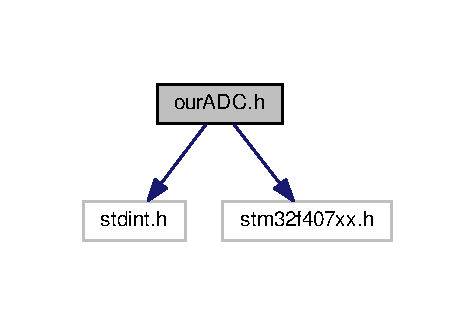
\includegraphics[width=228pt]{our_a_d_c_8h__incl}
\end{center}
\end{figure}
This graph shows which files directly or indirectly include this file\+:
\nopagebreak
\begin{figure}[H]
\begin{center}
\leavevmode
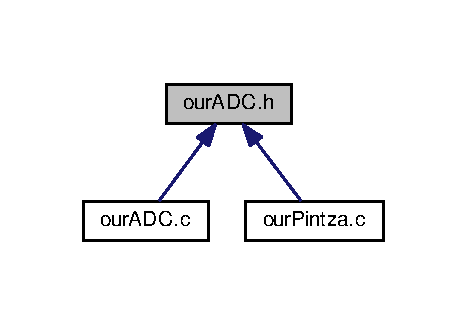
\includegraphics[width=224pt]{our_a_d_c_8h__dep__incl}
\end{center}
\end{figure}
\subsection*{Functions}
\begin{DoxyCompactItemize}
\item 
void \hyperlink{our_a_d_c_8h_a717656252b7f23c44aee8c93d8781965}{init\+A\+DC} (uint32\+\_\+t timer2\+T\+R\+GO, uint32\+\_\+t interrupzioa, uint32\+\_\+t kanala)
\item 
void \hyperlink{our_a_d_c_8h_a21c5d304a223b06f835851d581cbd697}{switch\+A\+DC} (int piztu)
\item 
uint16\+\_\+t \hyperlink{our_a_d_c_8h_aab4d2a3904f8b634c2ead90d0066c740}{get\+Azken\+Balioa} (void)
\item 
uint16\+\_\+t \hyperlink{our_a_d_c_8h_a38923b0842879b8f18e204a2cec0e67a}{get\+Balioa} (void)
\item 
void \hyperlink{our_a_d_c_8h_aa54231074f0827327eb2147b9eeb5376}{our\+A\+D\+C\+Handler} (void)
\item 
void \hyperlink{our_a_d_c_8h_a443125cba6c904aa284362d5ff18d459}{set\+A\+D\+C\+Call\+Back} (void($\ast$funtzioa)(uint16\+\_\+t))
\end{DoxyCompactItemize}


\subsection{Function Documentation}
\index{our\+A\+D\+C.\+h@{our\+A\+D\+C.\+h}!get\+Azken\+Balioa@{get\+Azken\+Balioa}}
\index{get\+Azken\+Balioa@{get\+Azken\+Balioa}!our\+A\+D\+C.\+h@{our\+A\+D\+C.\+h}}
\subsubsection[{\texorpdfstring{get\+Azken\+Balioa(void)}{getAzkenBalioa(void)}}]{\setlength{\rightskip}{0pt plus 5cm}uint16\+\_\+t get\+Azken\+Balioa (
\begin{DoxyParamCaption}
\item[{void}]{}
\end{DoxyParamCaption}
)}\hypertarget{our_a_d_c_8h_aab4d2a3904f8b634c2ead90d0066c740}{}\label{our_a_d_c_8h_aab4d2a3904f8b634c2ead90d0066c740}
Function that returns the last value of A\+DC. \begin{DoxyReturn}{Returns}
azken\+Balioa\+: uint16\+\_\+t type A\+DC last value. 
\end{DoxyReturn}
\index{our\+A\+D\+C.\+h@{our\+A\+D\+C.\+h}!get\+Balioa@{get\+Balioa}}
\index{get\+Balioa@{get\+Balioa}!our\+A\+D\+C.\+h@{our\+A\+D\+C.\+h}}
\subsubsection[{\texorpdfstring{get\+Balioa(void)}{getBalioa(void)}}]{\setlength{\rightskip}{0pt plus 5cm}uint16\+\_\+t get\+Balioa (
\begin{DoxyParamCaption}
\item[{void}]{}
\end{DoxyParamCaption}
)}\hypertarget{our_a_d_c_8h_a38923b0842879b8f18e204a2cec0e67a}{}\label{our_a_d_c_8h_a38923b0842879b8f18e204a2cec0e67a}
This function return the last value. \begin{DoxyReturn}{Returns}
azken\+Balioa\+: uint16\+\_\+t type conversion\textquotesingle{}s last value. 
\end{DoxyReturn}
\index{our\+A\+D\+C.\+h@{our\+A\+D\+C.\+h}!init\+A\+DC@{init\+A\+DC}}
\index{init\+A\+DC@{init\+A\+DC}!our\+A\+D\+C.\+h@{our\+A\+D\+C.\+h}}
\subsubsection[{\texorpdfstring{init\+A\+D\+C(uint32\+\_\+t timer2\+T\+R\+G\+O, uint32\+\_\+t interrupzioa, uint32\+\_\+t kanala)}{initADC(uint32_t timer2TRGO, uint32_t interrupzioa, uint32_t kanala)}}]{\setlength{\rightskip}{0pt plus 5cm}void init\+A\+DC (
\begin{DoxyParamCaption}
\item[{uint32\+\_\+t}]{timer2\+T\+R\+GO, }
\item[{uint32\+\_\+t}]{interrupzioa, }
\item[{uint32\+\_\+t}]{kanala}
\end{DoxyParamCaption}
)}\hypertarget{our_a_d_c_8h_a717656252b7f23c44aee8c93d8781965}{}\label{our_a_d_c_8h_a717656252b7f23c44aee8c93d8781965}
This function initializes A\+DC, setting core basic params to launch A\+DC. Some of the params are optional configurations such as interruption and T\+R\+GO. 
\begin{DoxyParams}{Parameters}
{\em timer2\+T\+R\+GO} & uint32\+\_\+t type but acts as a boolean to know if timer 2\textquotesingle{}s T\+R\+GO is needed. \\
\hline
{\em interrupzioa} & uint32\+\_\+t type but acts as boolean to know if interruption is needed. \\
\hline
{\em kanala} & uint32\+\_\+t type holds the value of which channel should be used by the A\+DC. \\
\hline
\end{DoxyParams}
\begin{DoxyReturn}{Returns}
void. 
\end{DoxyReturn}
\index{our\+A\+D\+C.\+h@{our\+A\+D\+C.\+h}!our\+A\+D\+C\+Handler@{our\+A\+D\+C\+Handler}}
\index{our\+A\+D\+C\+Handler@{our\+A\+D\+C\+Handler}!our\+A\+D\+C.\+h@{our\+A\+D\+C.\+h}}
\subsubsection[{\texorpdfstring{our\+A\+D\+C\+Handler(void)}{ourADCHandler(void)}}]{\setlength{\rightskip}{0pt plus 5cm}void our\+A\+D\+C\+Handler (
\begin{DoxyParamCaption}
\item[{void}]{}
\end{DoxyParamCaption}
)}\hypertarget{our_a_d_c_8h_aa54231074f0827327eb2147b9eeb5376}{}\label{our_a_d_c_8h_aa54231074f0827327eb2147b9eeb5376}
This function acts as a handler for the interruption caused by the A\+DC. \begin{DoxyReturn}{Returns}
void. 
\end{DoxyReturn}
\index{our\+A\+D\+C.\+h@{our\+A\+D\+C.\+h}!set\+A\+D\+C\+Call\+Back@{set\+A\+D\+C\+Call\+Back}}
\index{set\+A\+D\+C\+Call\+Back@{set\+A\+D\+C\+Call\+Back}!our\+A\+D\+C.\+h@{our\+A\+D\+C.\+h}}
\subsubsection[{\texorpdfstring{set\+A\+D\+C\+Call\+Back(void($\ast$funtzioa)(uint16\+\_\+t))}{setADCCallBack(void(*funtzioa)(uint16_t))}}]{\setlength{\rightskip}{0pt plus 5cm}void set\+A\+D\+C\+Call\+Back (
\begin{DoxyParamCaption}
\item[{void($\ast$)(uint16\+\_\+t)}]{funtzioa}
\end{DoxyParamCaption}
)}\hypertarget{our_a_d_c_8h_a443125cba6c904aa284362d5ff18d459}{}\label{our_a_d_c_8h_a443125cba6c904aa284362d5ff18d459}
This function sets a pointer to another function which accepts a paramater of type uint16\+\_\+t. Callback funtcion.  funtzio\+: void type points to a function. \begin{DoxyReturn}{Returns}
void 
\end{DoxyReturn}
\index{our\+A\+D\+C.\+h@{our\+A\+D\+C.\+h}!switch\+A\+DC@{switch\+A\+DC}}
\index{switch\+A\+DC@{switch\+A\+DC}!our\+A\+D\+C.\+h@{our\+A\+D\+C.\+h}}
\subsubsection[{\texorpdfstring{switch\+A\+D\+C(int piztu)}{switchADC(int piztu)}}]{\setlength{\rightskip}{0pt plus 5cm}void switch\+A\+DC (
\begin{DoxyParamCaption}
\item[{int}]{piztu}
\end{DoxyParamCaption}
)}\hypertarget{our_a_d_c_8h_a21c5d304a223b06f835851d581cbd697}{}\label{our_a_d_c_8h_a21c5d304a223b06f835851d581cbd697}
This function enable or disable A\+DC peripheral depending on the given parameter that acts as a boolean type. 
\begin{DoxyParams}{Parameters}
{\em piztu} & int type but acts as a boolean to know whether is needed to enable or disable A\+D\+C1. \\
\hline
\end{DoxyParams}
\begin{DoxyReturn}{Returns}
void. 
\end{DoxyReturn}

\hypertarget{our_d_a_c_8c}{}\section{our\+D\+A\+C.\+c File Reference}
\label{our_d_a_c_8c}\index{our\+D\+A\+C.\+c@{our\+D\+A\+C.\+c}}
{\ttfamily \#include \char`\"{}our\+D\+A\+C.\+h\char`\"{}}\\*
Include dependency graph for our\+D\+A\+C.\+c\+:
\nopagebreak
\begin{figure}[H]
\begin{center}
\leavevmode
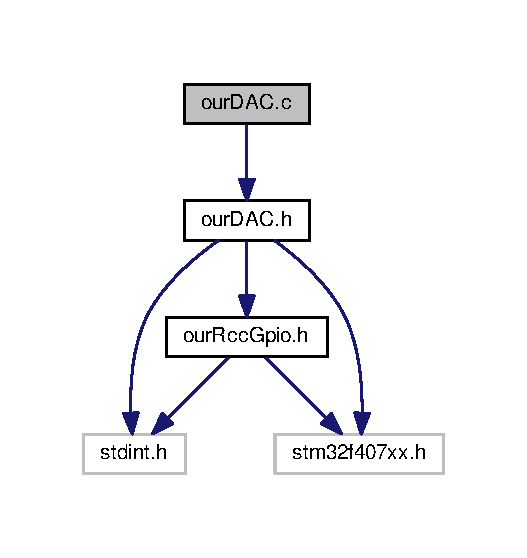
\includegraphics[width=253pt]{our_d_a_c_8c__incl}
\end{center}
\end{figure}
\subsection*{Functions}
\begin{DoxyCompactItemize}
\item 
void \hyperlink{our_d_a_c_8c_a2fbd396554513d0c125c80f942424498}{init\+G\+P\+I\+O\+D\+A\+C2} (void)
\item 
void \hyperlink{our_d_a_c_8c_a9f49e6b348374b0c2812f629f549d951}{init\+D\+AC} (uint32\+\_\+t dma, uint32\+\_\+t trgo2)
\item 
void \hyperlink{our_d_a_c_8c_a06ef5a63867df9c4f4a6fe60e4276330}{set\+Balioa} (uint32\+\_\+t balioa)
\end{DoxyCompactItemize}


\subsection{Function Documentation}
\index{our\+D\+A\+C.\+c@{our\+D\+A\+C.\+c}!init\+D\+AC@{init\+D\+AC}}
\index{init\+D\+AC@{init\+D\+AC}!our\+D\+A\+C.\+c@{our\+D\+A\+C.\+c}}
\subsubsection[{\texorpdfstring{init\+D\+A\+C(uint32\+\_\+t dma, uint32\+\_\+t trgo2)}{initDAC(uint32_t dma, uint32_t trgo2)}}]{\setlength{\rightskip}{0pt plus 5cm}void init\+D\+AC (
\begin{DoxyParamCaption}
\item[{uint32\+\_\+t}]{dma, }
\item[{uint32\+\_\+t}]{trgo2}
\end{DoxyParamCaption}
)}\hypertarget{our_d_a_c_8c_a9f49e6b348374b0c2812f629f549d951}{}\label{our_d_a_c_8c_a9f49e6b348374b0c2812f629f549d951}
\index{our\+D\+A\+C.\+c@{our\+D\+A\+C.\+c}!init\+G\+P\+I\+O\+D\+A\+C2@{init\+G\+P\+I\+O\+D\+A\+C2}}
\index{init\+G\+P\+I\+O\+D\+A\+C2@{init\+G\+P\+I\+O\+D\+A\+C2}!our\+D\+A\+C.\+c@{our\+D\+A\+C.\+c}}
\subsubsection[{\texorpdfstring{init\+G\+P\+I\+O\+D\+A\+C2(void)}{initGPIODAC2(void)}}]{\setlength{\rightskip}{0pt plus 5cm}void init\+G\+P\+I\+O\+D\+A\+C2 (
\begin{DoxyParamCaption}
\item[{void}]{}
\end{DoxyParamCaption}
)}\hypertarget{our_d_a_c_8c_a2fbd396554513d0c125c80f942424498}{}\label{our_d_a_c_8c_a2fbd396554513d0c125c80f942424498}
\index{our\+D\+A\+C.\+c@{our\+D\+A\+C.\+c}!set\+Balioa@{set\+Balioa}}
\index{set\+Balioa@{set\+Balioa}!our\+D\+A\+C.\+c@{our\+D\+A\+C.\+c}}
\subsubsection[{\texorpdfstring{set\+Balioa(uint32\+\_\+t balioa)}{setBalioa(uint32_t balioa)}}]{\setlength{\rightskip}{0pt plus 5cm}void set\+Balioa (
\begin{DoxyParamCaption}
\item[{uint32\+\_\+t}]{balioa}
\end{DoxyParamCaption}
)}\hypertarget{our_d_a_c_8c_a06ef5a63867df9c4f4a6fe60e4276330}{}\label{our_d_a_c_8c_a06ef5a63867df9c4f4a6fe60e4276330}

\hypertarget{our_d_a_c_8h}{}\section{our\+D\+A\+C.\+h File Reference}
\label{our_d_a_c_8h}\index{our\+D\+A\+C.\+h@{our\+D\+A\+C.\+h}}
{\ttfamily \#include $<$stdint.\+h$>$}\\*
{\ttfamily \#include \char`\"{}our\+Rcc\+Gpio.\+h\char`\"{}}\\*
{\ttfamily \#include $<$stm32f407xx.\+h$>$}\\*
Include dependency graph for our\+D\+A\+C.\+h\+:
\nopagebreak
\begin{figure}[H]
\begin{center}
\leavevmode
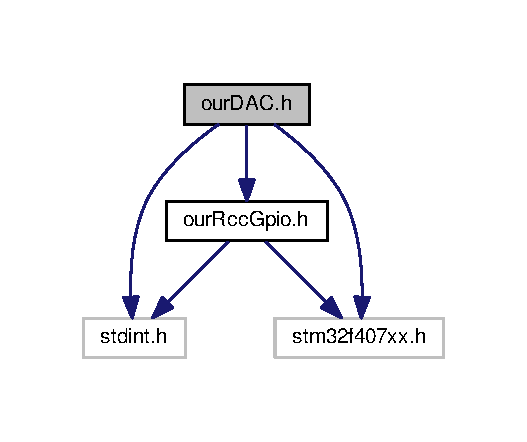
\includegraphics[width=253pt]{our_d_a_c_8h__incl}
\end{center}
\end{figure}
This graph shows which files directly or indirectly include this file\+:
\nopagebreak
\begin{figure}[H]
\begin{center}
\leavevmode
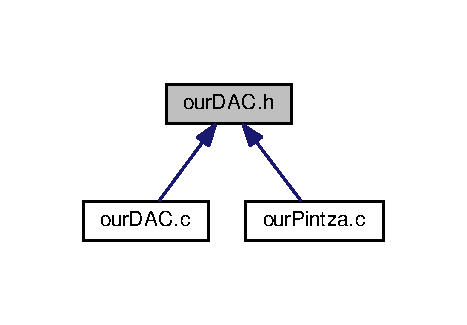
\includegraphics[width=224pt]{our_d_a_c_8h__dep__incl}
\end{center}
\end{figure}
\subsection*{Functions}
\begin{DoxyCompactItemize}
\item 
void \hyperlink{our_d_a_c_8h_a9f49e6b348374b0c2812f629f549d951}{init\+D\+AC} (uint32\+\_\+t dma, uint32\+\_\+t trgo2)
\item 
void \hyperlink{our_d_a_c_8h_a06ef5a63867df9c4f4a6fe60e4276330}{set\+Balioa} (uint32\+\_\+t balioa)
\end{DoxyCompactItemize}


\subsection{Function Documentation}
\index{our\+D\+A\+C.\+h@{our\+D\+A\+C.\+h}!init\+D\+AC@{init\+D\+AC}}
\index{init\+D\+AC@{init\+D\+AC}!our\+D\+A\+C.\+h@{our\+D\+A\+C.\+h}}
\subsubsection[{\texorpdfstring{init\+D\+A\+C(uint32\+\_\+t dma, uint32\+\_\+t trgo2)}{initDAC(uint32_t dma, uint32_t trgo2)}}]{\setlength{\rightskip}{0pt plus 5cm}void init\+D\+AC (
\begin{DoxyParamCaption}
\item[{uint32\+\_\+t}]{dma, }
\item[{uint32\+\_\+t}]{trgo2}
\end{DoxyParamCaption}
)}\hypertarget{our_d_a_c_8h_a9f49e6b348374b0c2812f629f549d951}{}\label{our_d_a_c_8h_a9f49e6b348374b0c2812f629f549d951}
\index{our\+D\+A\+C.\+h@{our\+D\+A\+C.\+h}!set\+Balioa@{set\+Balioa}}
\index{set\+Balioa@{set\+Balioa}!our\+D\+A\+C.\+h@{our\+D\+A\+C.\+h}}
\subsubsection[{\texorpdfstring{set\+Balioa(uint32\+\_\+t balioa)}{setBalioa(uint32_t balioa)}}]{\setlength{\rightskip}{0pt plus 5cm}void set\+Balioa (
\begin{DoxyParamCaption}
\item[{uint32\+\_\+t}]{balioa}
\end{DoxyParamCaption}
)}\hypertarget{our_d_a_c_8h_a06ef5a63867df9c4f4a6fe60e4276330}{}\label{our_d_a_c_8h_a06ef5a63867df9c4f4a6fe60e4276330}

\hypertarget{our_d_m_a_8c}{}\section{our\+D\+M\+A.\+c File Reference}
\label{our_d_m_a_8c}\index{our\+D\+M\+A.\+c@{our\+D\+M\+A.\+c}}
{\ttfamily \#include \char`\"{}our\+D\+M\+A.\+h\char`\"{}}\\*
Include dependency graph for our\+D\+M\+A.\+c\+:
\nopagebreak
\begin{figure}[H]
\begin{center}
\leavevmode
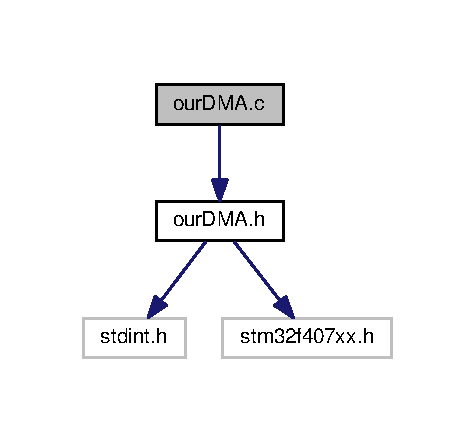
\includegraphics[width=228pt]{our_d_m_a_8c__incl}
\end{center}
\end{figure}
\subsection*{Functions}
\begin{DoxyCompactItemize}
\item 
void \hyperlink{our_d_m_a_8c_a35a61d30afff8549e6aa5f9acd02888d}{init\+D\+M\+A2\+D\+AC} (uint16\+\_\+t $\ast$emaitza)
\end{DoxyCompactItemize}


\subsection{Function Documentation}
\index{our\+D\+M\+A.\+c@{our\+D\+M\+A.\+c}!init\+D\+M\+A2\+D\+AC@{init\+D\+M\+A2\+D\+AC}}
\index{init\+D\+M\+A2\+D\+AC@{init\+D\+M\+A2\+D\+AC}!our\+D\+M\+A.\+c@{our\+D\+M\+A.\+c}}
\subsubsection[{\texorpdfstring{init\+D\+M\+A2\+D\+A\+C(uint16\+\_\+t $\ast$emaitza)}{initDMA2DAC(uint16_t *emaitza)}}]{\setlength{\rightskip}{0pt plus 5cm}void init\+D\+M\+A2\+D\+AC (
\begin{DoxyParamCaption}
\item[{uint16\+\_\+t $\ast$}]{emaitza}
\end{DoxyParamCaption}
)}\hypertarget{our_d_m_a_8c_a35a61d30afff8549e6aa5f9acd02888d}{}\label{our_d_m_a_8c_a35a61d30afff8549e6aa5f9acd02888d}

\hypertarget{our_d_m_a_8h}{}\section{our\+D\+M\+A.\+h File Reference}
\label{our_d_m_a_8h}\index{our\+D\+M\+A.\+h@{our\+D\+M\+A.\+h}}
{\ttfamily \#include $<$stdint.\+h$>$}\\*
{\ttfamily \#include $<$stm32f407xx.\+h$>$}\\*
Include dependency graph for our\+D\+M\+A.\+h\+:
\nopagebreak
\begin{figure}[H]
\begin{center}
\leavevmode
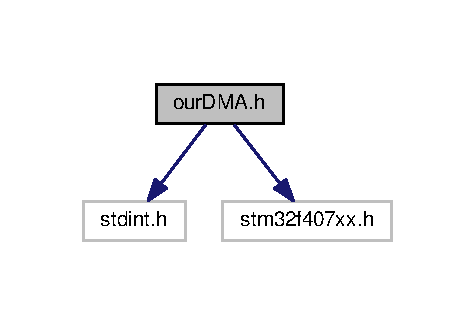
\includegraphics[width=228pt]{our_d_m_a_8h__incl}
\end{center}
\end{figure}
This graph shows which files directly or indirectly include this file\+:
\nopagebreak
\begin{figure}[H]
\begin{center}
\leavevmode
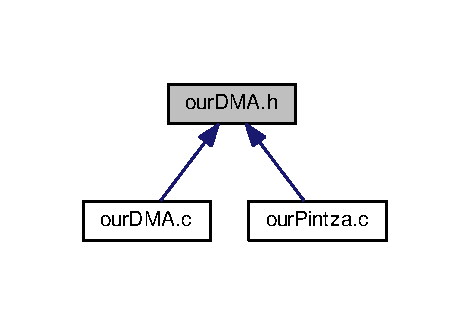
\includegraphics[width=226pt]{our_d_m_a_8h__dep__incl}
\end{center}
\end{figure}
\subsection*{Functions}
\begin{DoxyCompactItemize}
\item 
void \hyperlink{our_d_m_a_8h_a35a61d30afff8549e6aa5f9acd02888d}{init\+D\+M\+A2\+D\+AC} (uint16\+\_\+t $\ast$emaitza)
\end{DoxyCompactItemize}


\subsection{Function Documentation}
\index{our\+D\+M\+A.\+h@{our\+D\+M\+A.\+h}!init\+D\+M\+A2\+D\+AC@{init\+D\+M\+A2\+D\+AC}}
\index{init\+D\+M\+A2\+D\+AC@{init\+D\+M\+A2\+D\+AC}!our\+D\+M\+A.\+h@{our\+D\+M\+A.\+h}}
\subsubsection[{\texorpdfstring{init\+D\+M\+A2\+D\+A\+C(uint16\+\_\+t $\ast$emaitza)}{initDMA2DAC(uint16_t *emaitza)}}]{\setlength{\rightskip}{0pt plus 5cm}void init\+D\+M\+A2\+D\+AC (
\begin{DoxyParamCaption}
\item[{uint16\+\_\+t $\ast$}]{emaitza}
\end{DoxyParamCaption}
)}\hypertarget{our_d_m_a_8h_a35a61d30afff8549e6aa5f9acd02888d}{}\label{our_d_m_a_8h_a35a61d30afff8549e6aa5f9acd02888d}

\hypertarget{our_pintza_8c}{}\section{our\+Pintza.\+c File Reference}
\label{our_pintza_8c}\index{our\+Pintza.\+c@{our\+Pintza.\+c}}
{\ttfamily \#include \char`\"{}our\+Pintza.\+h\char`\"{}}\\*
{\ttfamily \#include \char`\"{}our\+A\+D\+C.\+h\char`\"{}}\\*
{\ttfamily \#include \char`\"{}our\+Timer.\+h\char`\"{}}\\*
{\ttfamily \#include \char`\"{}our\+Rcc\+Gpio.\+h\char`\"{}}\\*
{\ttfamily \#include \char`\"{}our\+D\+M\+A.\+h\char`\"{}}\\*
{\ttfamily \#include \char`\"{}our\+D\+A\+C.\+h\char`\"{}}\\*
Include dependency graph for our\+Pintza.\+c\+:
\nopagebreak
\begin{figure}[H]
\begin{center}
\leavevmode
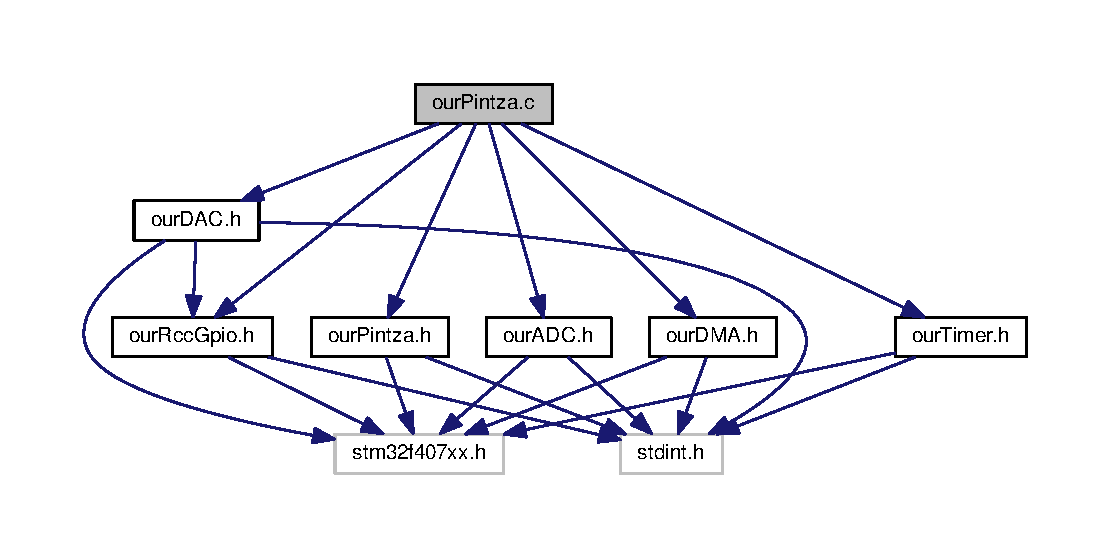
\includegraphics[width=350pt]{our_pintza_8c__incl}
\end{center}
\end{figure}
\subsection*{Macros}
\begin{DoxyCompactItemize}
\item 
\#define \hyperlink{our_pintza_8c_ae16276a6cb76cf1a1462573259174e2d}{Z\+I\+K\+L\+O\+\_\+\+K\+OP}~100
\item 
\#define \hyperlink{our_pintza_8c_adc88080d4f406a8f4cf0efe3c395688a}{T\+I\+M\+E\+R\+\_\+\+A\+B\+I\+A\+D\+U\+RA}~10
\item 
\#define \hyperlink{our_pintza_8c_a21005f9f4e2ce7597c5eb4351816d7e2}{O\+F\+F\+S\+ET}~(uint16\+\_\+t) 0x04d9
\end{DoxyCompactItemize}
\subsection*{Functions}
\begin{DoxyCompactItemize}
\item 
void \hyperlink{our_pintza_8c_a197488db1e4921e50419bde04a61b890}{A\+D\+Ccallback} (uint16\+\_\+t balioa)
\item 
void \hyperlink{our_pintza_8c_a9baabb03427960524df4a2fbb04f2e07}{init\+G\+P\+I\+O\+A6} (void)
\item 
void \hyperlink{our_pintza_8c_a62aa285aa159785a4686a5ac86ca8967}{init\+Pintza} (void)
\item 
void \hyperlink{our_pintza_8c_abb5ef8f5f79abfdadae9fd2de7d8ddb4}{power\+Pintza} (uint32\+\_\+t piztu)
\item 
uint16\+\_\+t \hyperlink{our_pintza_8c_a82fa6c5b99bf057573150a0609d8003c}{get\+Azken\+Kontsumoa} ()
\item 
void \hyperlink{our_pintza_8c_a071cd75f04cd5217e7cef31c901e2bee}{set\+Pintza\+Callback} (void($\ast$funtzioa)(uint16\+\_\+t))
\end{DoxyCompactItemize}
\subsection*{Variables}
\begin{DoxyCompactItemize}
\item 
uint16\+\_\+t \hyperlink{our_pintza_8c_afbf22e2955f0f34f2c76f425ce6cf272}{max\+Balioa} = 0
\item 
uint32\+\_\+t \hyperlink{our_pintza_8c_a10f57d5c143288292b4a59f189b02c01}{zikloak} = 0
\item 
uint16\+\_\+t \hyperlink{our_pintza_8c_afe29f7be5c2ee604debe235d6e5eac72}{azken\+Max\+Balioa} = 0
\item 
void($\ast$ \hyperlink{our_pintza_8c_a652b2248682b933712868addf6195852}{callback\+Pintza} )(uint16\+\_\+t)=0
\end{DoxyCompactItemize}


\subsection{Macro Definition Documentation}
\index{our\+Pintza.\+c@{our\+Pintza.\+c}!O\+F\+F\+S\+ET@{O\+F\+F\+S\+ET}}
\index{O\+F\+F\+S\+ET@{O\+F\+F\+S\+ET}!our\+Pintza.\+c@{our\+Pintza.\+c}}
\subsubsection[{\texorpdfstring{O\+F\+F\+S\+ET}{OFFSET}}]{\setlength{\rightskip}{0pt plus 5cm}\#define O\+F\+F\+S\+ET~(uint16\+\_\+t) 0x04d9}\hypertarget{our_pintza_8c_a21005f9f4e2ce7597c5eb4351816d7e2}{}\label{our_pintza_8c_a21005f9f4e2ce7597c5eb4351816d7e2}
\index{our\+Pintza.\+c@{our\+Pintza.\+c}!T\+I\+M\+E\+R\+\_\+\+A\+B\+I\+A\+D\+U\+RA@{T\+I\+M\+E\+R\+\_\+\+A\+B\+I\+A\+D\+U\+RA}}
\index{T\+I\+M\+E\+R\+\_\+\+A\+B\+I\+A\+D\+U\+RA@{T\+I\+M\+E\+R\+\_\+\+A\+B\+I\+A\+D\+U\+RA}!our\+Pintza.\+c@{our\+Pintza.\+c}}
\subsubsection[{\texorpdfstring{T\+I\+M\+E\+R\+\_\+\+A\+B\+I\+A\+D\+U\+RA}{TIMER_ABIADURA}}]{\setlength{\rightskip}{0pt plus 5cm}\#define T\+I\+M\+E\+R\+\_\+\+A\+B\+I\+A\+D\+U\+RA~10}\hypertarget{our_pintza_8c_adc88080d4f406a8f4cf0efe3c395688a}{}\label{our_pintza_8c_adc88080d4f406a8f4cf0efe3c395688a}
\index{our\+Pintza.\+c@{our\+Pintza.\+c}!Z\+I\+K\+L\+O\+\_\+\+K\+OP@{Z\+I\+K\+L\+O\+\_\+\+K\+OP}}
\index{Z\+I\+K\+L\+O\+\_\+\+K\+OP@{Z\+I\+K\+L\+O\+\_\+\+K\+OP}!our\+Pintza.\+c@{our\+Pintza.\+c}}
\subsubsection[{\texorpdfstring{Z\+I\+K\+L\+O\+\_\+\+K\+OP}{ZIKLO_KOP}}]{\setlength{\rightskip}{0pt plus 5cm}\#define Z\+I\+K\+L\+O\+\_\+\+K\+OP~100}\hypertarget{our_pintza_8c_ae16276a6cb76cf1a1462573259174e2d}{}\label{our_pintza_8c_ae16276a6cb76cf1a1462573259174e2d}


\subsection{Function Documentation}
\index{our\+Pintza.\+c@{our\+Pintza.\+c}!A\+D\+Ccallback@{A\+D\+Ccallback}}
\index{A\+D\+Ccallback@{A\+D\+Ccallback}!our\+Pintza.\+c@{our\+Pintza.\+c}}
\subsubsection[{\texorpdfstring{A\+D\+Ccallback(uint16\+\_\+t balioa)}{ADCcallback(uint16_t balioa)}}]{\setlength{\rightskip}{0pt plus 5cm}void A\+D\+Ccallback (
\begin{DoxyParamCaption}
\item[{uint16\+\_\+t}]{balioa}
\end{DoxyParamCaption}
)}\hypertarget{our_pintza_8c_a197488db1e4921e50419bde04a61b890}{}\label{our_pintza_8c_a197488db1e4921e50419bde04a61b890}
This function calculates the max value converted by the A\+DC. It waits for 3000 cycles and takes the max value. Used to take the peak value of the alternate current. And sets the max value to the callback function. 
\begin{DoxyParams}{Parameters}
{\em balio} & uint16\+\_\+t type current value converted by the A\+DC. \\
\hline
\end{DoxyParams}
\begin{DoxyReturn}{Returns}
void. 
\end{DoxyReturn}
\index{our\+Pintza.\+c@{our\+Pintza.\+c}!get\+Azken\+Kontsumoa@{get\+Azken\+Kontsumoa}}
\index{get\+Azken\+Kontsumoa@{get\+Azken\+Kontsumoa}!our\+Pintza.\+c@{our\+Pintza.\+c}}
\subsubsection[{\texorpdfstring{get\+Azken\+Kontsumoa()}{getAzkenKontsumoa()}}]{\setlength{\rightskip}{0pt plus 5cm}uint16\+\_\+t get\+Azken\+Kontsumoa (
\begin{DoxyParamCaption}
\item[{void}]{}
\end{DoxyParamCaption}
)}\hypertarget{our_pintza_8c_a82fa6c5b99bf057573150a0609d8003c}{}\label{our_pintza_8c_a82fa6c5b99bf057573150a0609d8003c}
Gets the last value from the conversion made by A\+DC. \begin{DoxyReturn}{Returns}
azken\+Balio\+: uint16\+\_\+t type last conversion value. 
\end{DoxyReturn}
\index{our\+Pintza.\+c@{our\+Pintza.\+c}!init\+G\+P\+I\+O\+A6@{init\+G\+P\+I\+O\+A6}}
\index{init\+G\+P\+I\+O\+A6@{init\+G\+P\+I\+O\+A6}!our\+Pintza.\+c@{our\+Pintza.\+c}}
\subsubsection[{\texorpdfstring{init\+G\+P\+I\+O\+A6(void)}{initGPIOA6(void)}}]{\setlength{\rightskip}{0pt plus 5cm}void init\+G\+P\+I\+O\+A6 (
\begin{DoxyParamCaption}
\item[{void}]{}
\end{DoxyParamCaption}
)}\hypertarget{our_pintza_8c_a9baabb03427960524df4a2fbb04f2e07}{}\label{our_pintza_8c_a9baabb03427960524df4a2fbb04f2e07}
Initializes G\+P\+I\+O6 and sets its mode to Analog mode. \begin{DoxyReturn}{Returns}
void. 
\end{DoxyReturn}
\index{our\+Pintza.\+c@{our\+Pintza.\+c}!init\+Pintza@{init\+Pintza}}
\index{init\+Pintza@{init\+Pintza}!our\+Pintza.\+c@{our\+Pintza.\+c}}
\subsubsection[{\texorpdfstring{init\+Pintza(void)}{initPintza(void)}}]{\setlength{\rightskip}{0pt plus 5cm}void init\+Pintza (
\begin{DoxyParamCaption}
\item[{void}]{}
\end{DoxyParamCaption}
)}\hypertarget{our_pintza_8c_a62aa285aa159785a4686a5ac86ca8967}{}\label{our_pintza_8c_a62aa285aa159785a4686a5ac86ca8967}
This function initializes some peripherals to work with an extern tool (pintza). Initializes G\+P\+I\+O6, Timer 2, A\+DC, D\+AC and D\+MA. \begin{DoxyReturn}{Returns}
void. 
\end{DoxyReturn}
\index{our\+Pintza.\+c@{our\+Pintza.\+c}!power\+Pintza@{power\+Pintza}}
\index{power\+Pintza@{power\+Pintza}!our\+Pintza.\+c@{our\+Pintza.\+c}}
\subsubsection[{\texorpdfstring{power\+Pintza(uint32\+\_\+t piztu)}{powerPintza(uint32_t piztu)}}]{\setlength{\rightskip}{0pt plus 5cm}void power\+Pintza (
\begin{DoxyParamCaption}
\item[{uint32\+\_\+t}]{piztu}
\end{DoxyParamCaption}
)}\hypertarget{our_pintza_8c_abb5ef8f5f79abfdadae9fd2de7d8ddb4}{}\label{our_pintza_8c_abb5ef8f5f79abfdadae9fd2de7d8ddb4}
This function enables or disables Timer2 and A\+DC depending on the given param. 
\begin{DoxyParams}{Parameters}
{\em piztu} & uint32\+\_\+t type acts as a boolean to enable or disable Timer 2 and A\+DC. \\
\hline
\end{DoxyParams}
\begin{DoxyReturn}{Returns}
void. 
\end{DoxyReturn}
\index{our\+Pintza.\+c@{our\+Pintza.\+c}!set\+Pintza\+Callback@{set\+Pintza\+Callback}}
\index{set\+Pintza\+Callback@{set\+Pintza\+Callback}!our\+Pintza.\+c@{our\+Pintza.\+c}}
\subsubsection[{\texorpdfstring{set\+Pintza\+Callback(void($\ast$funtzioa)(uint16\+\_\+t))}{setPintzaCallback(void(*funtzioa)(uint16_t))}}]{\setlength{\rightskip}{0pt plus 5cm}void set\+Pintza\+Callback (
\begin{DoxyParamCaption}
\item[{void($\ast$)(uint16\+\_\+t)}]{funtzioa}
\end{DoxyParamCaption}
)}\hypertarget{our_pintza_8c_a071cd75f04cd5217e7cef31c901e2bee}{}\label{our_pintza_8c_a071cd75f04cd5217e7cef31c901e2bee}
Sets callback function that recieves the last value of the conversion as parameter. 
\begin{DoxyParams}{Parameters}
{\em funtzioa} & void type function, is a pointer to a void returning function which take uint16\+\_\+t type parameter. \\
\hline
\end{DoxyParams}
\begin{DoxyReturn}{Returns}
void. 
\end{DoxyReturn}


\subsection{Variable Documentation}
\index{our\+Pintza.\+c@{our\+Pintza.\+c}!azken\+Max\+Balioa@{azken\+Max\+Balioa}}
\index{azken\+Max\+Balioa@{azken\+Max\+Balioa}!our\+Pintza.\+c@{our\+Pintza.\+c}}
\subsubsection[{\texorpdfstring{azken\+Max\+Balioa}{azkenMaxBalioa}}]{\setlength{\rightskip}{0pt plus 5cm}uint16\+\_\+t azken\+Max\+Balioa = 0}\hypertarget{our_pintza_8c_afe29f7be5c2ee604debe235d6e5eac72}{}\label{our_pintza_8c_afe29f7be5c2ee604debe235d6e5eac72}
\index{our\+Pintza.\+c@{our\+Pintza.\+c}!callback\+Pintza@{callback\+Pintza}}
\index{callback\+Pintza@{callback\+Pintza}!our\+Pintza.\+c@{our\+Pintza.\+c}}
\subsubsection[{\texorpdfstring{callback\+Pintza}{callbackPintza}}]{\setlength{\rightskip}{0pt plus 5cm}void($\ast$ callback\+Pintza) (uint16\+\_\+t)=0}\hypertarget{our_pintza_8c_a652b2248682b933712868addf6195852}{}\label{our_pintza_8c_a652b2248682b933712868addf6195852}
\index{our\+Pintza.\+c@{our\+Pintza.\+c}!max\+Balioa@{max\+Balioa}}
\index{max\+Balioa@{max\+Balioa}!our\+Pintza.\+c@{our\+Pintza.\+c}}
\subsubsection[{\texorpdfstring{max\+Balioa}{maxBalioa}}]{\setlength{\rightskip}{0pt plus 5cm}uint16\+\_\+t max\+Balioa = 0}\hypertarget{our_pintza_8c_afbf22e2955f0f34f2c76f425ce6cf272}{}\label{our_pintza_8c_afbf22e2955f0f34f2c76f425ce6cf272}
\index{our\+Pintza.\+c@{our\+Pintza.\+c}!zikloak@{zikloak}}
\index{zikloak@{zikloak}!our\+Pintza.\+c@{our\+Pintza.\+c}}
\subsubsection[{\texorpdfstring{zikloak}{zikloak}}]{\setlength{\rightskip}{0pt plus 5cm}uint32\+\_\+t zikloak = 0}\hypertarget{our_pintza_8c_a10f57d5c143288292b4a59f189b02c01}{}\label{our_pintza_8c_a10f57d5c143288292b4a59f189b02c01}

\hypertarget{our_pintza_8h}{}\section{our\+Pintza.\+h File Reference}
\label{our_pintza_8h}\index{our\+Pintza.\+h@{our\+Pintza.\+h}}
{\ttfamily \#include $<$stdint.\+h$>$}\\*
{\ttfamily \#include $<$stm32f407xx.\+h$>$}\\*
Include dependency graph for our\+Pintza.\+h\+:
\nopagebreak
\begin{figure}[H]
\begin{center}
\leavevmode
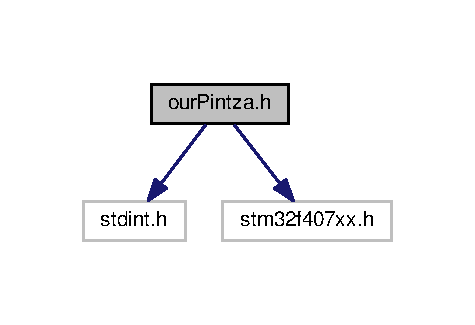
\includegraphics[width=228pt]{our_pintza_8h__incl}
\end{center}
\end{figure}
This graph shows which files directly or indirectly include this file\+:
\nopagebreak
\begin{figure}[H]
\begin{center}
\leavevmode
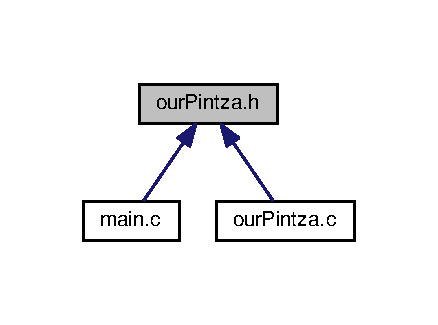
\includegraphics[width=210pt]{our_pintza_8h__dep__incl}
\end{center}
\end{figure}
\subsection*{Functions}
\begin{DoxyCompactItemize}
\item 
void \hyperlink{our_pintza_8h_a62aa285aa159785a4686a5ac86ca8967}{init\+Pintza} (void)
\item 
void \hyperlink{our_pintza_8h_abb5ef8f5f79abfdadae9fd2de7d8ddb4}{power\+Pintza} (uint32\+\_\+t piztu)
\item 
uint16\+\_\+t \hyperlink{our_pintza_8h_afba47c27a1a9ff05e11dda920353819a}{get\+Azken\+Kontsumoa} (void)
\item 
void \hyperlink{our_pintza_8h_a071cd75f04cd5217e7cef31c901e2bee}{set\+Pintza\+Callback} (void($\ast$funtzioa)(uint16\+\_\+t))
\item 
void \hyperlink{our_pintza_8h_a197488db1e4921e50419bde04a61b890}{A\+D\+Ccallback} (uint16\+\_\+t balioa)
\end{DoxyCompactItemize}


\subsection{Function Documentation}
\index{our\+Pintza.\+h@{our\+Pintza.\+h}!A\+D\+Ccallback@{A\+D\+Ccallback}}
\index{A\+D\+Ccallback@{A\+D\+Ccallback}!our\+Pintza.\+h@{our\+Pintza.\+h}}
\subsubsection[{\texorpdfstring{A\+D\+Ccallback(uint16\+\_\+t balioa)}{ADCcallback(uint16_t balioa)}}]{\setlength{\rightskip}{0pt plus 5cm}void A\+D\+Ccallback (
\begin{DoxyParamCaption}
\item[{uint16\+\_\+t}]{balioa}
\end{DoxyParamCaption}
)}\hypertarget{our_pintza_8h_a197488db1e4921e50419bde04a61b890}{}\label{our_pintza_8h_a197488db1e4921e50419bde04a61b890}
This function calculates the max value converted by the A\+DC. It waits for 3000 cycles and takes the max value. Used to take the peak value of the alternate current. And sets the max value to the callback function. 
\begin{DoxyParams}{Parameters}
{\em balio} & uint16\+\_\+t type current value converted by the A\+DC. \\
\hline
\end{DoxyParams}
\begin{DoxyReturn}{Returns}
void. 
\end{DoxyReturn}
\index{our\+Pintza.\+h@{our\+Pintza.\+h}!get\+Azken\+Kontsumoa@{get\+Azken\+Kontsumoa}}
\index{get\+Azken\+Kontsumoa@{get\+Azken\+Kontsumoa}!our\+Pintza.\+h@{our\+Pintza.\+h}}
\subsubsection[{\texorpdfstring{get\+Azken\+Kontsumoa(void)}{getAzkenKontsumoa(void)}}]{\setlength{\rightskip}{0pt plus 5cm}uint16\+\_\+t get\+Azken\+Kontsumoa (
\begin{DoxyParamCaption}
\item[{void}]{}
\end{DoxyParamCaption}
)}\hypertarget{our_pintza_8h_afba47c27a1a9ff05e11dda920353819a}{}\label{our_pintza_8h_afba47c27a1a9ff05e11dda920353819a}
Gets the last value from the conversion made by A\+DC. \begin{DoxyReturn}{Returns}
azken\+Balio\+: uint16\+\_\+t type last conversion value. 
\end{DoxyReturn}
\index{our\+Pintza.\+h@{our\+Pintza.\+h}!init\+Pintza@{init\+Pintza}}
\index{init\+Pintza@{init\+Pintza}!our\+Pintza.\+h@{our\+Pintza.\+h}}
\subsubsection[{\texorpdfstring{init\+Pintza(void)}{initPintza(void)}}]{\setlength{\rightskip}{0pt plus 5cm}void init\+Pintza (
\begin{DoxyParamCaption}
\item[{void}]{}
\end{DoxyParamCaption}
)}\hypertarget{our_pintza_8h_a62aa285aa159785a4686a5ac86ca8967}{}\label{our_pintza_8h_a62aa285aa159785a4686a5ac86ca8967}
This function initializes some peripherals to work with an extern tool (pintza). Initializes G\+P\+I\+O6, Timer 2, A\+DC, D\+AC and D\+MA. \begin{DoxyReturn}{Returns}
void. 
\end{DoxyReturn}
\index{our\+Pintza.\+h@{our\+Pintza.\+h}!power\+Pintza@{power\+Pintza}}
\index{power\+Pintza@{power\+Pintza}!our\+Pintza.\+h@{our\+Pintza.\+h}}
\subsubsection[{\texorpdfstring{power\+Pintza(uint32\+\_\+t piztu)}{powerPintza(uint32_t piztu)}}]{\setlength{\rightskip}{0pt plus 5cm}void power\+Pintza (
\begin{DoxyParamCaption}
\item[{uint32\+\_\+t}]{piztu}
\end{DoxyParamCaption}
)}\hypertarget{our_pintza_8h_abb5ef8f5f79abfdadae9fd2de7d8ddb4}{}\label{our_pintza_8h_abb5ef8f5f79abfdadae9fd2de7d8ddb4}
This function enables or disables Timer2 and A\+DC depending on the given param. 
\begin{DoxyParams}{Parameters}
{\em piztu} & uint32\+\_\+t type acts as a boolean to enable or disable Timer 2 and A\+DC. \\
\hline
\end{DoxyParams}
\begin{DoxyReturn}{Returns}
void. 
\end{DoxyReturn}
\index{our\+Pintza.\+h@{our\+Pintza.\+h}!set\+Pintza\+Callback@{set\+Pintza\+Callback}}
\index{set\+Pintza\+Callback@{set\+Pintza\+Callback}!our\+Pintza.\+h@{our\+Pintza.\+h}}
\subsubsection[{\texorpdfstring{set\+Pintza\+Callback(void($\ast$funtzioa)(uint16\+\_\+t))}{setPintzaCallback(void(*funtzioa)(uint16_t))}}]{\setlength{\rightskip}{0pt plus 5cm}void set\+Pintza\+Callback (
\begin{DoxyParamCaption}
\item[{void($\ast$)(uint16\+\_\+t)}]{funtzioa}
\end{DoxyParamCaption}
)}\hypertarget{our_pintza_8h_a071cd75f04cd5217e7cef31c901e2bee}{}\label{our_pintza_8h_a071cd75f04cd5217e7cef31c901e2bee}
Sets callback function that recieves the last value of the conversion as parameter. 
\begin{DoxyParams}{Parameters}
{\em funtzioa} & void type function, is a pointer to a void returning function which take uint16\+\_\+t type parameter. \\
\hline
\end{DoxyParams}
\begin{DoxyReturn}{Returns}
void. 
\end{DoxyReturn}

\hypertarget{our_rcc_gpio_8c}{}\section{our\+Rcc\+Gpio.\+c File Reference}
\label{our_rcc_gpio_8c}\index{our\+Rcc\+Gpio.\+c@{our\+Rcc\+Gpio.\+c}}
{\ttfamily \#include \char`\"{}our\+Rcc\+Gpio.\+h\char`\"{}}\\*
Include dependency graph for our\+Rcc\+Gpio.\+c\+:
\nopagebreak
\begin{figure}[H]
\begin{center}
\leavevmode
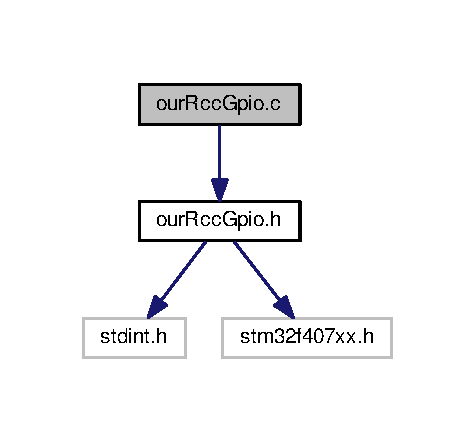
\includegraphics[width=228pt]{our_rcc_gpio_8c__incl}
\end{center}
\end{figure}
\subsection*{Functions}
\begin{DoxyCompactItemize}
\item 
void \hyperlink{our_rcc_gpio_8c_ad0e3f7bff9289ce46ddaafb13ce19f3d}{R\+C\+C\+\_\+\+A\+H\+B1\+Periph\+Clock\+Cmd} (uint32\+\_\+t n\+Periph, uint32\+\_\+t on)
\item 
void \hyperlink{our_rcc_gpio_8c_a7543dd4c0dc608ba3dfee05aa830de88}{R\+C\+C\+\_\+\+A\+H\+B1\+A\+P\+B2\+Periph\+Clock\+Cmd} (uint32\+\_\+t n\+Periph, uint32\+\_\+t on)
\item 
void \hyperlink{our_rcc_gpio_8c_a90c4f2b397b09475dd77a12d6fe1b007}{init\+Gpio\+Pin\+Mode} (G\+P\+I\+O\+\_\+\+Type\+Def $\ast$gpio, uint32\+\_\+t pin, \hyperlink{our_rcc_gpio_8h_aaba48df2a76dd7f822436358145cb6bb}{G\+P\+I\+O\+Mode\+\_\+\+Type} mode)
\item 
void \hyperlink{our_rcc_gpio_8c_a177dfc7c394712b34fcbb5cbcfabe86a}{togle\+Gpio\+Pin\+Value} (G\+P\+I\+O\+\_\+\+Type\+Def $\ast$gpio, uint32\+\_\+t pin)
\item 
void \hyperlink{our_rcc_gpio_8c_ad44a2224cef652252303ac71a56e84c3}{set\+Gpio\+Pin\+Value} (G\+P\+I\+O\+\_\+\+Type\+Def $\ast$gpio, uint32\+\_\+t pin, uint32\+\_\+t value)
\item 
uint32\+\_\+t \hyperlink{our_rcc_gpio_8c_ad3c36019126dbd3c6de7ccd4ec5f048d}{get\+Gpio\+Pin\+Value} (G\+P\+I\+O\+\_\+\+Type\+Def $\ast$gpio, uint32\+\_\+t pin)
\item 
void \hyperlink{our_rcc_gpio_8c_a00402e8c2c926e493d0a1399fc7cf765}{set\+Gpio\+Pin\+AF} (G\+P\+I\+O\+\_\+\+Type\+Def $\ast$gpio, uint32\+\_\+t pin, uint32\+\_\+t AF)
\end{DoxyCompactItemize}


\subsection{Function Documentation}
\index{our\+Rcc\+Gpio.\+c@{our\+Rcc\+Gpio.\+c}!get\+Gpio\+Pin\+Value@{get\+Gpio\+Pin\+Value}}
\index{get\+Gpio\+Pin\+Value@{get\+Gpio\+Pin\+Value}!our\+Rcc\+Gpio.\+c@{our\+Rcc\+Gpio.\+c}}
\subsubsection[{\texorpdfstring{get\+Gpio\+Pin\+Value(\+G\+P\+I\+O\+\_\+\+Type\+Def $\ast$gpio, uint32\+\_\+t pin)}{getGpioPinValue(GPIO_TypeDef *gpio, uint32_t pin)}}]{\setlength{\rightskip}{0pt plus 5cm}uint32\+\_\+t get\+Gpio\+Pin\+Value (
\begin{DoxyParamCaption}
\item[{G\+P\+I\+O\+\_\+\+Type\+Def $\ast$}]{gpio, }
\item[{uint32\+\_\+t}]{pin}
\end{DoxyParamCaption}
)}\hypertarget{our_rcc_gpio_8c_ad3c36019126dbd3c6de7ccd4ec5f048d}{}\label{our_rcc_gpio_8c_ad3c36019126dbd3c6de7ccd4ec5f048d}
\index{our\+Rcc\+Gpio.\+c@{our\+Rcc\+Gpio.\+c}!init\+Gpio\+Pin\+Mode@{init\+Gpio\+Pin\+Mode}}
\index{init\+Gpio\+Pin\+Mode@{init\+Gpio\+Pin\+Mode}!our\+Rcc\+Gpio.\+c@{our\+Rcc\+Gpio.\+c}}
\subsubsection[{\texorpdfstring{init\+Gpio\+Pin\+Mode(\+G\+P\+I\+O\+\_\+\+Type\+Def $\ast$gpio, uint32\+\_\+t pin, G\+P\+I\+O\+Mode\+\_\+\+Type mode)}{initGpioPinMode(GPIO_TypeDef *gpio, uint32_t pin, GPIOMode_Type mode)}}]{\setlength{\rightskip}{0pt plus 5cm}void init\+Gpio\+Pin\+Mode (
\begin{DoxyParamCaption}
\item[{G\+P\+I\+O\+\_\+\+Type\+Def $\ast$}]{gpio, }
\item[{uint32\+\_\+t}]{pin, }
\item[{{\bf G\+P\+I\+O\+Mode\+\_\+\+Type}}]{mode}
\end{DoxyParamCaption}
)}\hypertarget{our_rcc_gpio_8c_a90c4f2b397b09475dd77a12d6fe1b007}{}\label{our_rcc_gpio_8c_a90c4f2b397b09475dd77a12d6fe1b007}
\index{our\+Rcc\+Gpio.\+c@{our\+Rcc\+Gpio.\+c}!R\+C\+C\+\_\+\+A\+H\+B1\+A\+P\+B2\+Periph\+Clock\+Cmd@{R\+C\+C\+\_\+\+A\+H\+B1\+A\+P\+B2\+Periph\+Clock\+Cmd}}
\index{R\+C\+C\+\_\+\+A\+H\+B1\+A\+P\+B2\+Periph\+Clock\+Cmd@{R\+C\+C\+\_\+\+A\+H\+B1\+A\+P\+B2\+Periph\+Clock\+Cmd}!our\+Rcc\+Gpio.\+c@{our\+Rcc\+Gpio.\+c}}
\subsubsection[{\texorpdfstring{R\+C\+C\+\_\+\+A\+H\+B1\+A\+P\+B2\+Periph\+Clock\+Cmd(uint32\+\_\+t n\+Periph, uint32\+\_\+t on)}{RCC_AHB1APB2PeriphClockCmd(uint32_t nPeriph, uint32_t on)}}]{\setlength{\rightskip}{0pt plus 5cm}void R\+C\+C\+\_\+\+A\+H\+B1\+A\+P\+B2\+Periph\+Clock\+Cmd (
\begin{DoxyParamCaption}
\item[{uint32\+\_\+t}]{n\+Periph, }
\item[{uint32\+\_\+t}]{on}
\end{DoxyParamCaption}
)}\hypertarget{our_rcc_gpio_8c_a7543dd4c0dc608ba3dfee05aa830de88}{}\label{our_rcc_gpio_8c_a7543dd4c0dc608ba3dfee05aa830de88}
\index{our\+Rcc\+Gpio.\+c@{our\+Rcc\+Gpio.\+c}!R\+C\+C\+\_\+\+A\+H\+B1\+Periph\+Clock\+Cmd@{R\+C\+C\+\_\+\+A\+H\+B1\+Periph\+Clock\+Cmd}}
\index{R\+C\+C\+\_\+\+A\+H\+B1\+Periph\+Clock\+Cmd@{R\+C\+C\+\_\+\+A\+H\+B1\+Periph\+Clock\+Cmd}!our\+Rcc\+Gpio.\+c@{our\+Rcc\+Gpio.\+c}}
\subsubsection[{\texorpdfstring{R\+C\+C\+\_\+\+A\+H\+B1\+Periph\+Clock\+Cmd(uint32\+\_\+t n\+Periph, uint32\+\_\+t on)}{RCC_AHB1PeriphClockCmd(uint32_t nPeriph, uint32_t on)}}]{\setlength{\rightskip}{0pt plus 5cm}void R\+C\+C\+\_\+\+A\+H\+B1\+Periph\+Clock\+Cmd (
\begin{DoxyParamCaption}
\item[{uint32\+\_\+t}]{n\+Periph, }
\item[{uint32\+\_\+t}]{on}
\end{DoxyParamCaption}
)}\hypertarget{our_rcc_gpio_8c_ad0e3f7bff9289ce46ddaafb13ce19f3d}{}\label{our_rcc_gpio_8c_ad0e3f7bff9289ce46ddaafb13ce19f3d}
\index{our\+Rcc\+Gpio.\+c@{our\+Rcc\+Gpio.\+c}!set\+Gpio\+Pin\+AF@{set\+Gpio\+Pin\+AF}}
\index{set\+Gpio\+Pin\+AF@{set\+Gpio\+Pin\+AF}!our\+Rcc\+Gpio.\+c@{our\+Rcc\+Gpio.\+c}}
\subsubsection[{\texorpdfstring{set\+Gpio\+Pin\+A\+F(\+G\+P\+I\+O\+\_\+\+Type\+Def $\ast$gpio, uint32\+\_\+t pin, uint32\+\_\+t A\+F)}{setGpioPinAF(GPIO_TypeDef *gpio, uint32_t pin, uint32_t AF)}}]{\setlength{\rightskip}{0pt plus 5cm}void set\+Gpio\+Pin\+AF (
\begin{DoxyParamCaption}
\item[{G\+P\+I\+O\+\_\+\+Type\+Def $\ast$}]{gpio, }
\item[{uint32\+\_\+t}]{pin, }
\item[{uint32\+\_\+t}]{AF}
\end{DoxyParamCaption}
)}\hypertarget{our_rcc_gpio_8c_a00402e8c2c926e493d0a1399fc7cf765}{}\label{our_rcc_gpio_8c_a00402e8c2c926e493d0a1399fc7cf765}
\index{our\+Rcc\+Gpio.\+c@{our\+Rcc\+Gpio.\+c}!set\+Gpio\+Pin\+Value@{set\+Gpio\+Pin\+Value}}
\index{set\+Gpio\+Pin\+Value@{set\+Gpio\+Pin\+Value}!our\+Rcc\+Gpio.\+c@{our\+Rcc\+Gpio.\+c}}
\subsubsection[{\texorpdfstring{set\+Gpio\+Pin\+Value(\+G\+P\+I\+O\+\_\+\+Type\+Def $\ast$gpio, uint32\+\_\+t pin, uint32\+\_\+t value)}{setGpioPinValue(GPIO_TypeDef *gpio, uint32_t pin, uint32_t value)}}]{\setlength{\rightskip}{0pt plus 5cm}void set\+Gpio\+Pin\+Value (
\begin{DoxyParamCaption}
\item[{G\+P\+I\+O\+\_\+\+Type\+Def $\ast$}]{gpio, }
\item[{uint32\+\_\+t}]{pin, }
\item[{uint32\+\_\+t}]{value}
\end{DoxyParamCaption}
)}\hypertarget{our_rcc_gpio_8c_ad44a2224cef652252303ac71a56e84c3}{}\label{our_rcc_gpio_8c_ad44a2224cef652252303ac71a56e84c3}
\index{our\+Rcc\+Gpio.\+c@{our\+Rcc\+Gpio.\+c}!togle\+Gpio\+Pin\+Value@{togle\+Gpio\+Pin\+Value}}
\index{togle\+Gpio\+Pin\+Value@{togle\+Gpio\+Pin\+Value}!our\+Rcc\+Gpio.\+c@{our\+Rcc\+Gpio.\+c}}
\subsubsection[{\texorpdfstring{togle\+Gpio\+Pin\+Value(\+G\+P\+I\+O\+\_\+\+Type\+Def $\ast$gpio, uint32\+\_\+t pin)}{togleGpioPinValue(GPIO_TypeDef *gpio, uint32_t pin)}}]{\setlength{\rightskip}{0pt plus 5cm}void togle\+Gpio\+Pin\+Value (
\begin{DoxyParamCaption}
\item[{G\+P\+I\+O\+\_\+\+Type\+Def $\ast$}]{gpio, }
\item[{uint32\+\_\+t}]{pin}
\end{DoxyParamCaption}
)}\hypertarget{our_rcc_gpio_8c_a177dfc7c394712b34fcbb5cbcfabe86a}{}\label{our_rcc_gpio_8c_a177dfc7c394712b34fcbb5cbcfabe86a}

\hypertarget{our_rcc_gpio_8h}{}\section{our\+Rcc\+Gpio.\+h File Reference}
\label{our_rcc_gpio_8h}\index{our\+Rcc\+Gpio.\+h@{our\+Rcc\+Gpio.\+h}}
{\ttfamily \#include $<$stdint.\+h$>$}\\*
{\ttfamily \#include $<$stm32f407xx.\+h$>$}\\*
Include dependency graph for our\+Rcc\+Gpio.\+h\+:
\nopagebreak
\begin{figure}[H]
\begin{center}
\leavevmode
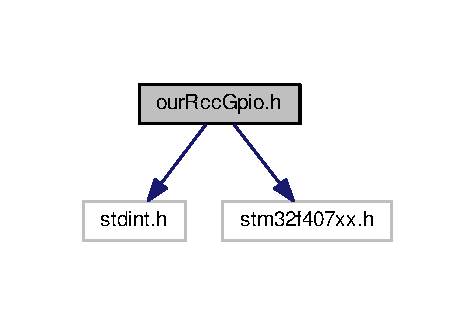
\includegraphics[width=228pt]{our_rcc_gpio_8h__incl}
\end{center}
\end{figure}
This graph shows which files directly or indirectly include this file\+:
\nopagebreak
\begin{figure}[H]
\begin{center}
\leavevmode
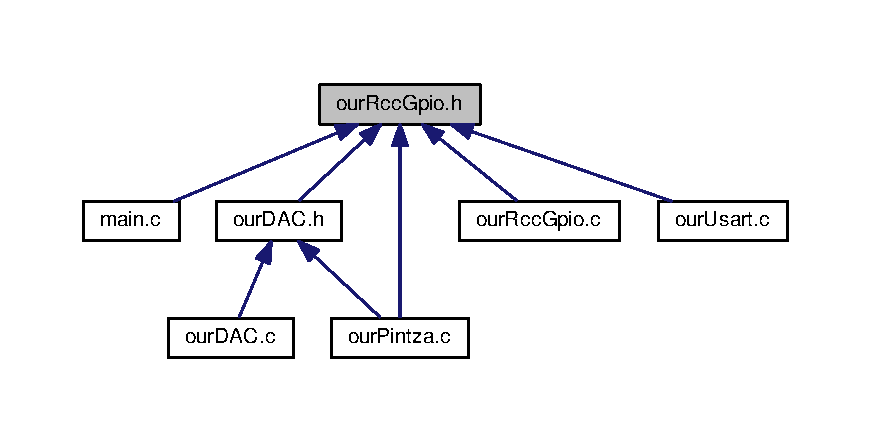
\includegraphics[width=350pt]{our_rcc_gpio_8h__dep__incl}
\end{center}
\end{figure}
\subsection*{Macros}
\begin{DoxyCompactItemize}
\item 
\#define \hyperlink{our_rcc_gpio_8h_a5196856bff085276016540e4c9c1dcf3}{R\+C\+C\+\_\+\+A\+H\+B1\+Periph\+\_\+\+G\+P\+I\+OA}~((uint32\+\_\+t)0x01)
\item 
\#define \hyperlink{our_rcc_gpio_8h_a41aceda5be7d382dd5fa321f5ca5c32f}{R\+C\+C\+\_\+\+A\+H\+B1\+Periph\+\_\+\+G\+P\+I\+OC}~((uint32\+\_\+t)(0x01$<$$<$2))
\item 
\#define \hyperlink{our_rcc_gpio_8h_a8f2001b801c7fe584ea1f6e9ab5c3274}{R\+C\+C\+\_\+\+A\+H\+B1\+Periph\+\_\+\+G\+P\+I\+OF}~((uint32\+\_\+t)(0x01$<$$<$5))
\item 
\#define \hyperlink{our_rcc_gpio_8h_a1d8fb07f858f198aaff77c71675f175d}{R\+C\+C\+\_\+\+A\+H\+B1\+Periph\+\_\+\+G\+P\+I\+OD}~((uint32\+\_\+t)(0x01$<$$<$3))
\item 
\#define \hyperlink{our_rcc_gpio_8h_ac34a5382981f1c19834fde41f205cf06}{R\+C\+C\+\_\+\+A\+H\+B1\+A\+P\+B2\+Periph\+\_\+\+S\+Y\+S\+C\+FG}~((uint32\+\_\+t)(0x01$<$$<$14))
\end{DoxyCompactItemize}
\subsection*{Enumerations}
\begin{DoxyCompactItemize}
\item 
enum \hyperlink{our_rcc_gpio_8h_aaba48df2a76dd7f822436358145cb6bb}{G\+P\+I\+O\+Mode\+\_\+\+Type} \{ \hyperlink{our_rcc_gpio_8h_aaba48df2a76dd7f822436358145cb6bba484aa18a6156ce916049b334ba1839de}{G\+P\+I\+O\+\_\+\+Mode\+\_\+\+IN} = 0x00, 
\hyperlink{our_rcc_gpio_8h_aaba48df2a76dd7f822436358145cb6bba60f1d530f4119efcad8e1a68c890c6a6}{G\+P\+I\+O\+\_\+\+Mode\+\_\+\+O\+UT} = 0x01, 
\hyperlink{our_rcc_gpio_8h_aaba48df2a76dd7f822436358145cb6bba6d44c35c6c5008d85bac9251a867e701}{G\+P\+I\+O\+\_\+\+Mode\+\_\+\+AF} = 0x02, 
\hyperlink{our_rcc_gpio_8h_aaba48df2a76dd7f822436358145cb6bba6e5c0d7e6d2e22b834b24e1ca1d6d0db}{G\+P\+I\+O\+\_\+\+Mode\+\_\+\+AN} = 0x03
 \}
\end{DoxyCompactItemize}
\subsection*{Functions}
\begin{DoxyCompactItemize}
\item 
void \hyperlink{our_rcc_gpio_8h_ad0e3f7bff9289ce46ddaafb13ce19f3d}{R\+C\+C\+\_\+\+A\+H\+B1\+Periph\+Clock\+Cmd} (uint32\+\_\+t n\+Periph, uint32\+\_\+t on)
\item 
void \hyperlink{our_rcc_gpio_8h_a7543dd4c0dc608ba3dfee05aa830de88}{R\+C\+C\+\_\+\+A\+H\+B1\+A\+P\+B2\+Periph\+Clock\+Cmd} (uint32\+\_\+t n\+Periph, uint32\+\_\+t on)
\item 
void \hyperlink{our_rcc_gpio_8h_a66c8c156cd83707b8f4ad11c0ceb0655}{init\+Gpio\+Pin\+Mode} (G\+P\+I\+O\+\_\+\+Type\+Def $\ast$, uint32\+\_\+t pin, \hyperlink{our_rcc_gpio_8h_aaba48df2a76dd7f822436358145cb6bb}{G\+P\+I\+O\+Mode\+\_\+\+Type} mode)
\item 
void \hyperlink{our_rcc_gpio_8h_a1061e5e9c03acdff3237cc0a58d75941}{togle\+Gpio\+Pin\+Value} (G\+P\+I\+O\+\_\+\+Type\+Def $\ast$, uint32\+\_\+t pin)
\item 
void \hyperlink{our_rcc_gpio_8h_ab9e87b45373664db189ad357cc73e403}{set\+Gpio\+Pin\+Value} (G\+P\+I\+O\+\_\+\+Type\+Def $\ast$, uint32\+\_\+t pin, uint32\+\_\+t value)
\item 
uint32\+\_\+t \hyperlink{our_rcc_gpio_8h_a65ed28fa329a76aac1a927b07044f120}{get\+Gpio\+Pin\+Value} (G\+P\+I\+O\+\_\+\+Type\+Def $\ast$, uint32\+\_\+t pin)
\item 
void \hyperlink{our_rcc_gpio_8h_a00402e8c2c926e493d0a1399fc7cf765}{set\+Gpio\+Pin\+AF} (G\+P\+I\+O\+\_\+\+Type\+Def $\ast$gpio, uint32\+\_\+t pin, uint32\+\_\+t AF)
\end{DoxyCompactItemize}


\subsection{Macro Definition Documentation}
\index{our\+Rcc\+Gpio.\+h@{our\+Rcc\+Gpio.\+h}!R\+C\+C\+\_\+\+A\+H\+B1\+A\+P\+B2\+Periph\+\_\+\+S\+Y\+S\+C\+FG@{R\+C\+C\+\_\+\+A\+H\+B1\+A\+P\+B2\+Periph\+\_\+\+S\+Y\+S\+C\+FG}}
\index{R\+C\+C\+\_\+\+A\+H\+B1\+A\+P\+B2\+Periph\+\_\+\+S\+Y\+S\+C\+FG@{R\+C\+C\+\_\+\+A\+H\+B1\+A\+P\+B2\+Periph\+\_\+\+S\+Y\+S\+C\+FG}!our\+Rcc\+Gpio.\+h@{our\+Rcc\+Gpio.\+h}}
\subsubsection[{\texorpdfstring{R\+C\+C\+\_\+\+A\+H\+B1\+A\+P\+B2\+Periph\+\_\+\+S\+Y\+S\+C\+FG}{RCC_AHB1APB2Periph_SYSCFG}}]{\setlength{\rightskip}{0pt plus 5cm}\#define R\+C\+C\+\_\+\+A\+H\+B1\+A\+P\+B2\+Periph\+\_\+\+S\+Y\+S\+C\+FG~((uint32\+\_\+t)(0x01$<$$<$14))}\hypertarget{our_rcc_gpio_8h_ac34a5382981f1c19834fde41f205cf06}{}\label{our_rcc_gpio_8h_ac34a5382981f1c19834fde41f205cf06}
\index{our\+Rcc\+Gpio.\+h@{our\+Rcc\+Gpio.\+h}!R\+C\+C\+\_\+\+A\+H\+B1\+Periph\+\_\+\+G\+P\+I\+OA@{R\+C\+C\+\_\+\+A\+H\+B1\+Periph\+\_\+\+G\+P\+I\+OA}}
\index{R\+C\+C\+\_\+\+A\+H\+B1\+Periph\+\_\+\+G\+P\+I\+OA@{R\+C\+C\+\_\+\+A\+H\+B1\+Periph\+\_\+\+G\+P\+I\+OA}!our\+Rcc\+Gpio.\+h@{our\+Rcc\+Gpio.\+h}}
\subsubsection[{\texorpdfstring{R\+C\+C\+\_\+\+A\+H\+B1\+Periph\+\_\+\+G\+P\+I\+OA}{RCC_AHB1Periph_GPIOA}}]{\setlength{\rightskip}{0pt plus 5cm}\#define R\+C\+C\+\_\+\+A\+H\+B1\+Periph\+\_\+\+G\+P\+I\+OA~((uint32\+\_\+t)0x01)}\hypertarget{our_rcc_gpio_8h_a5196856bff085276016540e4c9c1dcf3}{}\label{our_rcc_gpio_8h_a5196856bff085276016540e4c9c1dcf3}
\index{our\+Rcc\+Gpio.\+h@{our\+Rcc\+Gpio.\+h}!R\+C\+C\+\_\+\+A\+H\+B1\+Periph\+\_\+\+G\+P\+I\+OC@{R\+C\+C\+\_\+\+A\+H\+B1\+Periph\+\_\+\+G\+P\+I\+OC}}
\index{R\+C\+C\+\_\+\+A\+H\+B1\+Periph\+\_\+\+G\+P\+I\+OC@{R\+C\+C\+\_\+\+A\+H\+B1\+Periph\+\_\+\+G\+P\+I\+OC}!our\+Rcc\+Gpio.\+h@{our\+Rcc\+Gpio.\+h}}
\subsubsection[{\texorpdfstring{R\+C\+C\+\_\+\+A\+H\+B1\+Periph\+\_\+\+G\+P\+I\+OC}{RCC_AHB1Periph_GPIOC}}]{\setlength{\rightskip}{0pt plus 5cm}\#define R\+C\+C\+\_\+\+A\+H\+B1\+Periph\+\_\+\+G\+P\+I\+OC~((uint32\+\_\+t)(0x01$<$$<$2))}\hypertarget{our_rcc_gpio_8h_a41aceda5be7d382dd5fa321f5ca5c32f}{}\label{our_rcc_gpio_8h_a41aceda5be7d382dd5fa321f5ca5c32f}
\index{our\+Rcc\+Gpio.\+h@{our\+Rcc\+Gpio.\+h}!R\+C\+C\+\_\+\+A\+H\+B1\+Periph\+\_\+\+G\+P\+I\+OD@{R\+C\+C\+\_\+\+A\+H\+B1\+Periph\+\_\+\+G\+P\+I\+OD}}
\index{R\+C\+C\+\_\+\+A\+H\+B1\+Periph\+\_\+\+G\+P\+I\+OD@{R\+C\+C\+\_\+\+A\+H\+B1\+Periph\+\_\+\+G\+P\+I\+OD}!our\+Rcc\+Gpio.\+h@{our\+Rcc\+Gpio.\+h}}
\subsubsection[{\texorpdfstring{R\+C\+C\+\_\+\+A\+H\+B1\+Periph\+\_\+\+G\+P\+I\+OD}{RCC_AHB1Periph_GPIOD}}]{\setlength{\rightskip}{0pt plus 5cm}\#define R\+C\+C\+\_\+\+A\+H\+B1\+Periph\+\_\+\+G\+P\+I\+OD~((uint32\+\_\+t)(0x01$<$$<$3))}\hypertarget{our_rcc_gpio_8h_a1d8fb07f858f198aaff77c71675f175d}{}\label{our_rcc_gpio_8h_a1d8fb07f858f198aaff77c71675f175d}
\index{our\+Rcc\+Gpio.\+h@{our\+Rcc\+Gpio.\+h}!R\+C\+C\+\_\+\+A\+H\+B1\+Periph\+\_\+\+G\+P\+I\+OF@{R\+C\+C\+\_\+\+A\+H\+B1\+Periph\+\_\+\+G\+P\+I\+OF}}
\index{R\+C\+C\+\_\+\+A\+H\+B1\+Periph\+\_\+\+G\+P\+I\+OF@{R\+C\+C\+\_\+\+A\+H\+B1\+Periph\+\_\+\+G\+P\+I\+OF}!our\+Rcc\+Gpio.\+h@{our\+Rcc\+Gpio.\+h}}
\subsubsection[{\texorpdfstring{R\+C\+C\+\_\+\+A\+H\+B1\+Periph\+\_\+\+G\+P\+I\+OF}{RCC_AHB1Periph_GPIOF}}]{\setlength{\rightskip}{0pt plus 5cm}\#define R\+C\+C\+\_\+\+A\+H\+B1\+Periph\+\_\+\+G\+P\+I\+OF~((uint32\+\_\+t)(0x01$<$$<$5))}\hypertarget{our_rcc_gpio_8h_a8f2001b801c7fe584ea1f6e9ab5c3274}{}\label{our_rcc_gpio_8h_a8f2001b801c7fe584ea1f6e9ab5c3274}


\subsection{Enumeration Type Documentation}
\index{our\+Rcc\+Gpio.\+h@{our\+Rcc\+Gpio.\+h}!G\+P\+I\+O\+Mode\+\_\+\+Type@{G\+P\+I\+O\+Mode\+\_\+\+Type}}
\index{G\+P\+I\+O\+Mode\+\_\+\+Type@{G\+P\+I\+O\+Mode\+\_\+\+Type}!our\+Rcc\+Gpio.\+h@{our\+Rcc\+Gpio.\+h}}
\subsubsection[{\texorpdfstring{G\+P\+I\+O\+Mode\+\_\+\+Type}{GPIOMode_Type}}]{\setlength{\rightskip}{0pt plus 5cm}enum {\bf G\+P\+I\+O\+Mode\+\_\+\+Type}}\hypertarget{our_rcc_gpio_8h_aaba48df2a76dd7f822436358145cb6bb}{}\label{our_rcc_gpio_8h_aaba48df2a76dd7f822436358145cb6bb}
\begin{Desc}
\item[Enumerator]\par
\begin{description}
\index{G\+P\+I\+O\+\_\+\+Mode\+\_\+\+IN@{G\+P\+I\+O\+\_\+\+Mode\+\_\+\+IN}!our\+Rcc\+Gpio.\+h@{our\+Rcc\+Gpio.\+h}}\index{our\+Rcc\+Gpio.\+h@{our\+Rcc\+Gpio.\+h}!G\+P\+I\+O\+\_\+\+Mode\+\_\+\+IN@{G\+P\+I\+O\+\_\+\+Mode\+\_\+\+IN}}\item[{\em 
G\+P\+I\+O\+\_\+\+Mode\+\_\+\+IN\hypertarget{our_rcc_gpio_8h_aaba48df2a76dd7f822436358145cb6bba484aa18a6156ce916049b334ba1839de}{}\label{our_rcc_gpio_8h_aaba48df2a76dd7f822436358145cb6bba484aa18a6156ce916049b334ba1839de}
}]G\+P\+IO Input Mode \index{G\+P\+I\+O\+\_\+\+Mode\+\_\+\+O\+UT@{G\+P\+I\+O\+\_\+\+Mode\+\_\+\+O\+UT}!our\+Rcc\+Gpio.\+h@{our\+Rcc\+Gpio.\+h}}\index{our\+Rcc\+Gpio.\+h@{our\+Rcc\+Gpio.\+h}!G\+P\+I\+O\+\_\+\+Mode\+\_\+\+O\+UT@{G\+P\+I\+O\+\_\+\+Mode\+\_\+\+O\+UT}}\item[{\em 
G\+P\+I\+O\+\_\+\+Mode\+\_\+\+O\+UT\hypertarget{our_rcc_gpio_8h_aaba48df2a76dd7f822436358145cb6bba60f1d530f4119efcad8e1a68c890c6a6}{}\label{our_rcc_gpio_8h_aaba48df2a76dd7f822436358145cb6bba60f1d530f4119efcad8e1a68c890c6a6}
}]G\+P\+IO Output Mode \index{G\+P\+I\+O\+\_\+\+Mode\+\_\+\+AF@{G\+P\+I\+O\+\_\+\+Mode\+\_\+\+AF}!our\+Rcc\+Gpio.\+h@{our\+Rcc\+Gpio.\+h}}\index{our\+Rcc\+Gpio.\+h@{our\+Rcc\+Gpio.\+h}!G\+P\+I\+O\+\_\+\+Mode\+\_\+\+AF@{G\+P\+I\+O\+\_\+\+Mode\+\_\+\+AF}}\item[{\em 
G\+P\+I\+O\+\_\+\+Mode\+\_\+\+AF\hypertarget{our_rcc_gpio_8h_aaba48df2a76dd7f822436358145cb6bba6d44c35c6c5008d85bac9251a867e701}{}\label{our_rcc_gpio_8h_aaba48df2a76dd7f822436358145cb6bba6d44c35c6c5008d85bac9251a867e701}
}]G\+P\+IO Alternate function Mode \index{G\+P\+I\+O\+\_\+\+Mode\+\_\+\+AN@{G\+P\+I\+O\+\_\+\+Mode\+\_\+\+AN}!our\+Rcc\+Gpio.\+h@{our\+Rcc\+Gpio.\+h}}\index{our\+Rcc\+Gpio.\+h@{our\+Rcc\+Gpio.\+h}!G\+P\+I\+O\+\_\+\+Mode\+\_\+\+AN@{G\+P\+I\+O\+\_\+\+Mode\+\_\+\+AN}}\item[{\em 
G\+P\+I\+O\+\_\+\+Mode\+\_\+\+AN\hypertarget{our_rcc_gpio_8h_aaba48df2a76dd7f822436358145cb6bba6e5c0d7e6d2e22b834b24e1ca1d6d0db}{}\label{our_rcc_gpio_8h_aaba48df2a76dd7f822436358145cb6bba6e5c0d7e6d2e22b834b24e1ca1d6d0db}
}]G\+P\+IO Analog Mode \end{description}
\end{Desc}


\subsection{Function Documentation}
\index{our\+Rcc\+Gpio.\+h@{our\+Rcc\+Gpio.\+h}!get\+Gpio\+Pin\+Value@{get\+Gpio\+Pin\+Value}}
\index{get\+Gpio\+Pin\+Value@{get\+Gpio\+Pin\+Value}!our\+Rcc\+Gpio.\+h@{our\+Rcc\+Gpio.\+h}}
\subsubsection[{\texorpdfstring{get\+Gpio\+Pin\+Value(\+G\+P\+I\+O\+\_\+\+Type\+Def $\ast$, uint32\+\_\+t pin)}{getGpioPinValue(GPIO_TypeDef *, uint32_t pin)}}]{\setlength{\rightskip}{0pt plus 5cm}uint32\+\_\+t get\+Gpio\+Pin\+Value (
\begin{DoxyParamCaption}
\item[{G\+P\+I\+O\+\_\+\+Type\+Def $\ast$}]{, }
\item[{uint32\+\_\+t}]{pin}
\end{DoxyParamCaption}
)}\hypertarget{our_rcc_gpio_8h_a65ed28fa329a76aac1a927b07044f120}{}\label{our_rcc_gpio_8h_a65ed28fa329a76aac1a927b07044f120}
\index{our\+Rcc\+Gpio.\+h@{our\+Rcc\+Gpio.\+h}!init\+Gpio\+Pin\+Mode@{init\+Gpio\+Pin\+Mode}}
\index{init\+Gpio\+Pin\+Mode@{init\+Gpio\+Pin\+Mode}!our\+Rcc\+Gpio.\+h@{our\+Rcc\+Gpio.\+h}}
\subsubsection[{\texorpdfstring{init\+Gpio\+Pin\+Mode(\+G\+P\+I\+O\+\_\+\+Type\+Def $\ast$, uint32\+\_\+t pin, G\+P\+I\+O\+Mode\+\_\+\+Type mode)}{initGpioPinMode(GPIO_TypeDef *, uint32_t pin, GPIOMode_Type mode)}}]{\setlength{\rightskip}{0pt plus 5cm}void init\+Gpio\+Pin\+Mode (
\begin{DoxyParamCaption}
\item[{G\+P\+I\+O\+\_\+\+Type\+Def $\ast$}]{, }
\item[{uint32\+\_\+t}]{pin, }
\item[{{\bf G\+P\+I\+O\+Mode\+\_\+\+Type}}]{mode}
\end{DoxyParamCaption}
)}\hypertarget{our_rcc_gpio_8h_a66c8c156cd83707b8f4ad11c0ceb0655}{}\label{our_rcc_gpio_8h_a66c8c156cd83707b8f4ad11c0ceb0655}
\index{our\+Rcc\+Gpio.\+h@{our\+Rcc\+Gpio.\+h}!R\+C\+C\+\_\+\+A\+H\+B1\+A\+P\+B2\+Periph\+Clock\+Cmd@{R\+C\+C\+\_\+\+A\+H\+B1\+A\+P\+B2\+Periph\+Clock\+Cmd}}
\index{R\+C\+C\+\_\+\+A\+H\+B1\+A\+P\+B2\+Periph\+Clock\+Cmd@{R\+C\+C\+\_\+\+A\+H\+B1\+A\+P\+B2\+Periph\+Clock\+Cmd}!our\+Rcc\+Gpio.\+h@{our\+Rcc\+Gpio.\+h}}
\subsubsection[{\texorpdfstring{R\+C\+C\+\_\+\+A\+H\+B1\+A\+P\+B2\+Periph\+Clock\+Cmd(uint32\+\_\+t n\+Periph, uint32\+\_\+t on)}{RCC_AHB1APB2PeriphClockCmd(uint32_t nPeriph, uint32_t on)}}]{\setlength{\rightskip}{0pt plus 5cm}void R\+C\+C\+\_\+\+A\+H\+B1\+A\+P\+B2\+Periph\+Clock\+Cmd (
\begin{DoxyParamCaption}
\item[{uint32\+\_\+t}]{n\+Periph, }
\item[{uint32\+\_\+t}]{on}
\end{DoxyParamCaption}
)}\hypertarget{our_rcc_gpio_8h_a7543dd4c0dc608ba3dfee05aa830de88}{}\label{our_rcc_gpio_8h_a7543dd4c0dc608ba3dfee05aa830de88}
\index{our\+Rcc\+Gpio.\+h@{our\+Rcc\+Gpio.\+h}!R\+C\+C\+\_\+\+A\+H\+B1\+Periph\+Clock\+Cmd@{R\+C\+C\+\_\+\+A\+H\+B1\+Periph\+Clock\+Cmd}}
\index{R\+C\+C\+\_\+\+A\+H\+B1\+Periph\+Clock\+Cmd@{R\+C\+C\+\_\+\+A\+H\+B1\+Periph\+Clock\+Cmd}!our\+Rcc\+Gpio.\+h@{our\+Rcc\+Gpio.\+h}}
\subsubsection[{\texorpdfstring{R\+C\+C\+\_\+\+A\+H\+B1\+Periph\+Clock\+Cmd(uint32\+\_\+t n\+Periph, uint32\+\_\+t on)}{RCC_AHB1PeriphClockCmd(uint32_t nPeriph, uint32_t on)}}]{\setlength{\rightskip}{0pt plus 5cm}void R\+C\+C\+\_\+\+A\+H\+B1\+Periph\+Clock\+Cmd (
\begin{DoxyParamCaption}
\item[{uint32\+\_\+t}]{n\+Periph, }
\item[{uint32\+\_\+t}]{on}
\end{DoxyParamCaption}
)}\hypertarget{our_rcc_gpio_8h_ad0e3f7bff9289ce46ddaafb13ce19f3d}{}\label{our_rcc_gpio_8h_ad0e3f7bff9289ce46ddaafb13ce19f3d}
\index{our\+Rcc\+Gpio.\+h@{our\+Rcc\+Gpio.\+h}!set\+Gpio\+Pin\+AF@{set\+Gpio\+Pin\+AF}}
\index{set\+Gpio\+Pin\+AF@{set\+Gpio\+Pin\+AF}!our\+Rcc\+Gpio.\+h@{our\+Rcc\+Gpio.\+h}}
\subsubsection[{\texorpdfstring{set\+Gpio\+Pin\+A\+F(\+G\+P\+I\+O\+\_\+\+Type\+Def $\ast$gpio, uint32\+\_\+t pin, uint32\+\_\+t A\+F)}{setGpioPinAF(GPIO_TypeDef *gpio, uint32_t pin, uint32_t AF)}}]{\setlength{\rightskip}{0pt plus 5cm}void set\+Gpio\+Pin\+AF (
\begin{DoxyParamCaption}
\item[{G\+P\+I\+O\+\_\+\+Type\+Def $\ast$}]{gpio, }
\item[{uint32\+\_\+t}]{pin, }
\item[{uint32\+\_\+t}]{AF}
\end{DoxyParamCaption}
)}\hypertarget{our_rcc_gpio_8h_a00402e8c2c926e493d0a1399fc7cf765}{}\label{our_rcc_gpio_8h_a00402e8c2c926e493d0a1399fc7cf765}
\index{our\+Rcc\+Gpio.\+h@{our\+Rcc\+Gpio.\+h}!set\+Gpio\+Pin\+Value@{set\+Gpio\+Pin\+Value}}
\index{set\+Gpio\+Pin\+Value@{set\+Gpio\+Pin\+Value}!our\+Rcc\+Gpio.\+h@{our\+Rcc\+Gpio.\+h}}
\subsubsection[{\texorpdfstring{set\+Gpio\+Pin\+Value(\+G\+P\+I\+O\+\_\+\+Type\+Def $\ast$, uint32\+\_\+t pin, uint32\+\_\+t value)}{setGpioPinValue(GPIO_TypeDef *, uint32_t pin, uint32_t value)}}]{\setlength{\rightskip}{0pt plus 5cm}void set\+Gpio\+Pin\+Value (
\begin{DoxyParamCaption}
\item[{G\+P\+I\+O\+\_\+\+Type\+Def $\ast$}]{, }
\item[{uint32\+\_\+t}]{pin, }
\item[{uint32\+\_\+t}]{value}
\end{DoxyParamCaption}
)}\hypertarget{our_rcc_gpio_8h_ab9e87b45373664db189ad357cc73e403}{}\label{our_rcc_gpio_8h_ab9e87b45373664db189ad357cc73e403}
\index{our\+Rcc\+Gpio.\+h@{our\+Rcc\+Gpio.\+h}!togle\+Gpio\+Pin\+Value@{togle\+Gpio\+Pin\+Value}}
\index{togle\+Gpio\+Pin\+Value@{togle\+Gpio\+Pin\+Value}!our\+Rcc\+Gpio.\+h@{our\+Rcc\+Gpio.\+h}}
\subsubsection[{\texorpdfstring{togle\+Gpio\+Pin\+Value(\+G\+P\+I\+O\+\_\+\+Type\+Def $\ast$, uint32\+\_\+t pin)}{togleGpioPinValue(GPIO_TypeDef *, uint32_t pin)}}]{\setlength{\rightskip}{0pt plus 5cm}void togle\+Gpio\+Pin\+Value (
\begin{DoxyParamCaption}
\item[{G\+P\+I\+O\+\_\+\+Type\+Def $\ast$}]{, }
\item[{uint32\+\_\+t}]{pin}
\end{DoxyParamCaption}
)}\hypertarget{our_rcc_gpio_8h_a1061e5e9c03acdff3237cc0a58d75941}{}\label{our_rcc_gpio_8h_a1061e5e9c03acdff3237cc0a58d75941}

\hypertarget{our_systick_8c}{}\section{our\+Systick.\+c File Reference}
\label{our_systick_8c}\index{our\+Systick.\+c@{our\+Systick.\+c}}
{\ttfamily \#include \char`\"{}our\+Systick.\+h\char`\"{}}\\*
Include dependency graph for our\+Systick.\+c\+:
\nopagebreak
\begin{figure}[H]
\begin{center}
\leavevmode
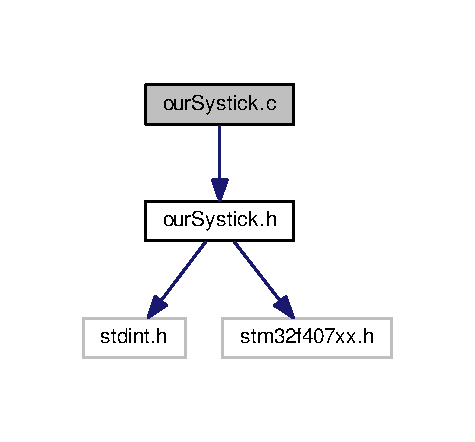
\includegraphics[width=228pt]{our_systick_8c__incl}
\end{center}
\end{figure}
\subsection*{Functions}
\begin{DoxyCompactItemize}
\item 
void \hyperlink{our_systick_8c_ac5ba5d23d61ca2e9a564ec6aad5221b4}{init\+Sys\+Tick} (uint32\+\_\+t ms, uint32\+\_\+t internal\+Clk)
\item 
uint32\+\_\+t \hyperlink{our_systick_8c_afa8f4dcf412151885ef146f574827b95}{get\+Sys\+Ticks} (void)
\item 
void \hyperlink{our_systick_8c_a19975fb04994a67d7ec95540d836b3dc}{wait\+Next\+Sys\+Tick} (void)
\item 
void \hyperlink{our_systick_8c_a1564f1e1bb9db6cffe092a31b7ee8c27}{our\+Sys\+Tick\+Handler} (void)
\end{DoxyCompactItemize}
\subsection*{Variables}
\begin{DoxyCompactItemize}
\item 
uint32\+\_\+t \hyperlink{our_systick_8c_ab9553772b4f58c24099f93aefe737100}{systicks} = 0
\item 
uint32\+\_\+t \hyperlink{our_systick_8c_ac3d00ec354cdb669d5b5768ec40429ac}{systick\+Old} = 0
\end{DoxyCompactItemize}


\subsection{Function Documentation}
\index{our\+Systick.\+c@{our\+Systick.\+c}!get\+Sys\+Ticks@{get\+Sys\+Ticks}}
\index{get\+Sys\+Ticks@{get\+Sys\+Ticks}!our\+Systick.\+c@{our\+Systick.\+c}}
\subsubsection[{\texorpdfstring{get\+Sys\+Ticks(void)}{getSysTicks(void)}}]{\setlength{\rightskip}{0pt plus 5cm}uint32\+\_\+t get\+Sys\+Ticks (
\begin{DoxyParamCaption}
\item[{void}]{}
\end{DoxyParamCaption}
)}\hypertarget{our_systick_8c_afa8f4dcf412151885ef146f574827b95}{}\label{our_systick_8c_afa8f4dcf412151885ef146f574827b95}
Get the current system tick value.  systicks\+: uint32\+\_\+t type ticks value. \index{our\+Systick.\+c@{our\+Systick.\+c}!init\+Sys\+Tick@{init\+Sys\+Tick}}
\index{init\+Sys\+Tick@{init\+Sys\+Tick}!our\+Systick.\+c@{our\+Systick.\+c}}
\subsubsection[{\texorpdfstring{init\+Sys\+Tick(uint32\+\_\+t ms, uint32\+\_\+t internal\+Clk)}{initSysTick(uint32_t ms, uint32_t internalClk)}}]{\setlength{\rightskip}{0pt plus 5cm}void init\+Sys\+Tick (
\begin{DoxyParamCaption}
\item[{uint32\+\_\+t}]{ms, }
\item[{uint32\+\_\+t}]{internal\+Clk}
\end{DoxyParamCaption}
)}\hypertarget{our_systick_8c_ac5ba5d23d61ca2e9a564ec6aad5221b4}{}\label{our_systick_8c_ac5ba5d23d61ca2e9a564ec6aad5221b4}
Initializes the System Tick core peripheral. 
\begin{DoxyParams}{Parameters}
{\em ms} & uint32\+\_\+t type sets the milliseconds for the clock \\
\hline
{\em internal\+Clk} & uint32\+\_\+t type optional parameter, acts as a boolean to know whether internal clock is needed. \\
\hline
\end{DoxyParams}
\begin{DoxyReturn}{Returns}
void. 
\end{DoxyReturn}
\index{our\+Systick.\+c@{our\+Systick.\+c}!our\+Sys\+Tick\+Handler@{our\+Sys\+Tick\+Handler}}
\index{our\+Sys\+Tick\+Handler@{our\+Sys\+Tick\+Handler}!our\+Systick.\+c@{our\+Systick.\+c}}
\subsubsection[{\texorpdfstring{our\+Sys\+Tick\+Handler(void)}{ourSysTickHandler(void)}}]{\setlength{\rightskip}{0pt plus 5cm}void our\+Sys\+Tick\+Handler (
\begin{DoxyParamCaption}
\item[{void}]{}
\end{DoxyParamCaption}
)}\hypertarget{our_systick_8c_a1564f1e1bb9db6cffe092a31b7ee8c27}{}\label{our_systick_8c_a1564f1e1bb9db6cffe092a31b7ee8c27}
Interruption handler for Sys\+Tick. \begin{DoxyReturn}{Returns}
void. 
\end{DoxyReturn}
\index{our\+Systick.\+c@{our\+Systick.\+c}!wait\+Next\+Sys\+Tick@{wait\+Next\+Sys\+Tick}}
\index{wait\+Next\+Sys\+Tick@{wait\+Next\+Sys\+Tick}!our\+Systick.\+c@{our\+Systick.\+c}}
\subsubsection[{\texorpdfstring{wait\+Next\+Sys\+Tick(void)}{waitNextSysTick(void)}}]{\setlength{\rightskip}{0pt plus 5cm}void wait\+Next\+Sys\+Tick (
\begin{DoxyParamCaption}
\item[{void}]{}
\end{DoxyParamCaption}
)}\hypertarget{our_systick_8c_a19975fb04994a67d7ec95540d836b3dc}{}\label{our_systick_8c_a19975fb04994a67d7ec95540d836b3dc}
This function is used to count until the next system tick. \begin{DoxyReturn}{Returns}
void. 
\end{DoxyReturn}


\subsection{Variable Documentation}
\index{our\+Systick.\+c@{our\+Systick.\+c}!systick\+Old@{systick\+Old}}
\index{systick\+Old@{systick\+Old}!our\+Systick.\+c@{our\+Systick.\+c}}
\subsubsection[{\texorpdfstring{systick\+Old}{systickOld}}]{\setlength{\rightskip}{0pt plus 5cm}uint32\+\_\+t systick\+Old = 0}\hypertarget{our_systick_8c_ac3d00ec354cdb669d5b5768ec40429ac}{}\label{our_systick_8c_ac3d00ec354cdb669d5b5768ec40429ac}
\index{our\+Systick.\+c@{our\+Systick.\+c}!systicks@{systicks}}
\index{systicks@{systicks}!our\+Systick.\+c@{our\+Systick.\+c}}
\subsubsection[{\texorpdfstring{systicks}{systicks}}]{\setlength{\rightskip}{0pt plus 5cm}uint32\+\_\+t systicks = 0}\hypertarget{our_systick_8c_ab9553772b4f58c24099f93aefe737100}{}\label{our_systick_8c_ab9553772b4f58c24099f93aefe737100}

\hypertarget{our_systick_8h}{}\section{our\+Systick.\+h File Reference}
\label{our_systick_8h}\index{our\+Systick.\+h@{our\+Systick.\+h}}
{\ttfamily \#include $<$stdint.\+h$>$}\\*
{\ttfamily \#include $<$stm32f407xx.\+h$>$}\\*
Include dependency graph for our\+Systick.\+h\+:
\nopagebreak
\begin{figure}[H]
\begin{center}
\leavevmode
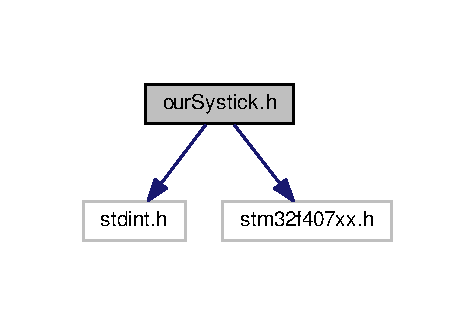
\includegraphics[width=228pt]{our_systick_8h__incl}
\end{center}
\end{figure}
This graph shows which files directly or indirectly include this file\+:
\nopagebreak
\begin{figure}[H]
\begin{center}
\leavevmode
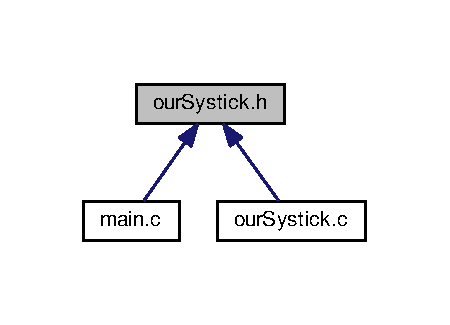
\includegraphics[width=216pt]{our_systick_8h__dep__incl}
\end{center}
\end{figure}
\subsection*{Functions}
\begin{DoxyCompactItemize}
\item 
void \hyperlink{our_systick_8h_ac5ba5d23d61ca2e9a564ec6aad5221b4}{init\+Sys\+Tick} (uint32\+\_\+t ms, uint32\+\_\+t internal\+Clk)
\item 
uint32\+\_\+t \hyperlink{our_systick_8h_afa8f4dcf412151885ef146f574827b95}{get\+Sys\+Ticks} (void)
\item 
void \hyperlink{our_systick_8h_a19975fb04994a67d7ec95540d836b3dc}{wait\+Next\+Sys\+Tick} (void)
\item 
void \hyperlink{our_systick_8h_a1564f1e1bb9db6cffe092a31b7ee8c27}{our\+Sys\+Tick\+Handler} (void)
\end{DoxyCompactItemize}


\subsection{Function Documentation}
\index{our\+Systick.\+h@{our\+Systick.\+h}!get\+Sys\+Ticks@{get\+Sys\+Ticks}}
\index{get\+Sys\+Ticks@{get\+Sys\+Ticks}!our\+Systick.\+h@{our\+Systick.\+h}}
\subsubsection[{\texorpdfstring{get\+Sys\+Ticks(void)}{getSysTicks(void)}}]{\setlength{\rightskip}{0pt plus 5cm}uint32\+\_\+t get\+Sys\+Ticks (
\begin{DoxyParamCaption}
\item[{void}]{}
\end{DoxyParamCaption}
)}\hypertarget{our_systick_8h_afa8f4dcf412151885ef146f574827b95}{}\label{our_systick_8h_afa8f4dcf412151885ef146f574827b95}
Get the current system tick value.  systicks\+: uint32\+\_\+t type ticks value. \index{our\+Systick.\+h@{our\+Systick.\+h}!init\+Sys\+Tick@{init\+Sys\+Tick}}
\index{init\+Sys\+Tick@{init\+Sys\+Tick}!our\+Systick.\+h@{our\+Systick.\+h}}
\subsubsection[{\texorpdfstring{init\+Sys\+Tick(uint32\+\_\+t ms, uint32\+\_\+t internal\+Clk)}{initSysTick(uint32_t ms, uint32_t internalClk)}}]{\setlength{\rightskip}{0pt plus 5cm}void init\+Sys\+Tick (
\begin{DoxyParamCaption}
\item[{uint32\+\_\+t}]{ms, }
\item[{uint32\+\_\+t}]{internal\+Clk}
\end{DoxyParamCaption}
)}\hypertarget{our_systick_8h_ac5ba5d23d61ca2e9a564ec6aad5221b4}{}\label{our_systick_8h_ac5ba5d23d61ca2e9a564ec6aad5221b4}
Initializes the System Tick core peripheral. 
\begin{DoxyParams}{Parameters}
{\em ms} & uint32\+\_\+t type sets the milliseconds for the clock \\
\hline
{\em internal\+Clk} & uint32\+\_\+t type optional parameter, acts as a boolean to know whether internal clock is needed. \\
\hline
\end{DoxyParams}
\begin{DoxyReturn}{Returns}
void. 
\end{DoxyReturn}
\index{our\+Systick.\+h@{our\+Systick.\+h}!our\+Sys\+Tick\+Handler@{our\+Sys\+Tick\+Handler}}
\index{our\+Sys\+Tick\+Handler@{our\+Sys\+Tick\+Handler}!our\+Systick.\+h@{our\+Systick.\+h}}
\subsubsection[{\texorpdfstring{our\+Sys\+Tick\+Handler(void)}{ourSysTickHandler(void)}}]{\setlength{\rightskip}{0pt plus 5cm}void our\+Sys\+Tick\+Handler (
\begin{DoxyParamCaption}
\item[{void}]{}
\end{DoxyParamCaption}
)}\hypertarget{our_systick_8h_a1564f1e1bb9db6cffe092a31b7ee8c27}{}\label{our_systick_8h_a1564f1e1bb9db6cffe092a31b7ee8c27}
Interruption handler for Sys\+Tick. \begin{DoxyReturn}{Returns}
void. 
\end{DoxyReturn}
\index{our\+Systick.\+h@{our\+Systick.\+h}!wait\+Next\+Sys\+Tick@{wait\+Next\+Sys\+Tick}}
\index{wait\+Next\+Sys\+Tick@{wait\+Next\+Sys\+Tick}!our\+Systick.\+h@{our\+Systick.\+h}}
\subsubsection[{\texorpdfstring{wait\+Next\+Sys\+Tick(void)}{waitNextSysTick(void)}}]{\setlength{\rightskip}{0pt plus 5cm}void wait\+Next\+Sys\+Tick (
\begin{DoxyParamCaption}
\item[{void}]{}
\end{DoxyParamCaption}
)}\hypertarget{our_systick_8h_a19975fb04994a67d7ec95540d836b3dc}{}\label{our_systick_8h_a19975fb04994a67d7ec95540d836b3dc}
This function is used to count until the next system tick. \begin{DoxyReturn}{Returns}
void. 
\end{DoxyReturn}

\hypertarget{our_timer_8c}{}\section{our\+Timer.\+c File Reference}
\label{our_timer_8c}\index{our\+Timer.\+c@{our\+Timer.\+c}}
{\ttfamily \#include \char`\"{}our\+Timer.\+h\char`\"{}}\\*
Include dependency graph for our\+Timer.\+c\+:
\nopagebreak
\begin{figure}[H]
\begin{center}
\leavevmode
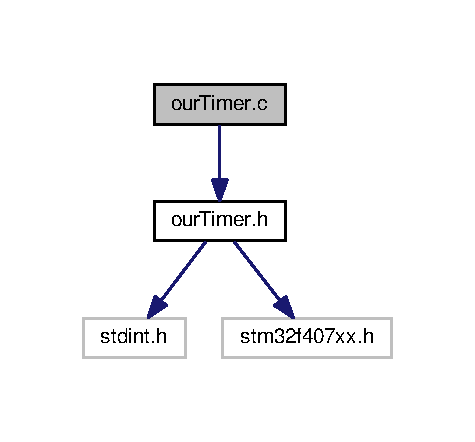
\includegraphics[width=228pt]{our_timer_8c__incl}
\end{center}
\end{figure}
\subsection*{Functions}
\begin{DoxyCompactItemize}
\item 
void \hyperlink{our_timer_8c_a4e742ad28873317354eb02338622cda4}{init\+Timer2} (uint32\+\_\+t ms, uint32\+\_\+t tr\+Go, uint32\+\_\+t interrupzioa)
\item 
void \hyperlink{our_timer_8c_aa7583a2b51bed765f33770ad8ec8b50e}{switch\+Timer2} (int piztu)
\item 
void \hyperlink{our_timer_8c_a984c824e117d7db294dc91fda4bb44f5}{wait\+Tick} (void)
\item 
uint32\+\_\+t \hyperlink{our_timer_8c_a4ac70252749c1e2a3006e0a76b5b9c6e}{get\+Ticks} (void)
\item 
void \hyperlink{our_timer_8c_a4b2ea4175a8cd1eb4d6934a46a69743f}{set\+Timer2\+Call\+Back} (void($\ast$funtzioa)(void))
\item 
void \hyperlink{our_timer_8c_a4d6ee62b5f61c89897eed1052296d104}{our\+Timer2\+Handler} (void)
\end{DoxyCompactItemize}
\subsection*{Variables}
\begin{DoxyCompactItemize}
\item 
void($\ast$ \hyperlink{our_timer_8c_a07db6e3e5f1b9d9468742d4960b51f3a}{callback\+Timer2} )(void)=0
\item 
volatile uint32\+\_\+t \hyperlink{our_timer_8c_aa7e25380b955a5364bf9bbd7f269cd00}{ticks} =0
\item 
volatile uint32\+\_\+t \hyperlink{our_timer_8c_aff1e2191cb0dbba93d6658954bc4eab4}{ticks\+Old} =0
\end{DoxyCompactItemize}


\subsection{Function Documentation}
\index{our\+Timer.\+c@{our\+Timer.\+c}!get\+Ticks@{get\+Ticks}}
\index{get\+Ticks@{get\+Ticks}!our\+Timer.\+c@{our\+Timer.\+c}}
\subsubsection[{\texorpdfstring{get\+Ticks(void)}{getTicks(void)}}]{\setlength{\rightskip}{0pt plus 5cm}uint32\+\_\+t get\+Ticks (
\begin{DoxyParamCaption}
\item[{void}]{}
\end{DoxyParamCaption}
)}\hypertarget{our_timer_8c_a4ac70252749c1e2a3006e0a76b5b9c6e}{}\label{our_timer_8c_a4ac70252749c1e2a3006e0a76b5b9c6e}
\index{our\+Timer.\+c@{our\+Timer.\+c}!init\+Timer2@{init\+Timer2}}
\index{init\+Timer2@{init\+Timer2}!our\+Timer.\+c@{our\+Timer.\+c}}
\subsubsection[{\texorpdfstring{init\+Timer2(uint32\+\_\+t ms, uint32\+\_\+t tr\+Go, uint32\+\_\+t interrupzioa)}{initTimer2(uint32_t ms, uint32_t trGo, uint32_t interrupzioa)}}]{\setlength{\rightskip}{0pt plus 5cm}void init\+Timer2 (
\begin{DoxyParamCaption}
\item[{uint32\+\_\+t}]{ms, }
\item[{uint32\+\_\+t}]{tr\+Go, }
\item[{uint32\+\_\+t}]{interrupzioa}
\end{DoxyParamCaption}
)}\hypertarget{our_timer_8c_a4e742ad28873317354eb02338622cda4}{}\label{our_timer_8c_a4e742ad28873317354eb02338622cda4}
Initializes timer 2 setting basic configurations for launch. Some given paramaters such as tr\+Go and interrupzio are optional. 
\begin{DoxyParams}{Parameters}
{\em ms} & uint32\+\_\+t type time in millisecond above which timer 2 have to operate. \\
\hline
{\em tr\+Go} & uint32\+\_\+t acts as boolean to know whether is needed to enable T\+R\+GO signal. \\
\hline
{\em interrupzioa} & uint32\+\_\+t acts as a boolean to know whether interruption configuration is needed. \\
\hline
\end{DoxyParams}
\begin{DoxyReturn}{Returns}
void. 
\end{DoxyReturn}
\index{our\+Timer.\+c@{our\+Timer.\+c}!our\+Timer2\+Handler@{our\+Timer2\+Handler}}
\index{our\+Timer2\+Handler@{our\+Timer2\+Handler}!our\+Timer.\+c@{our\+Timer.\+c}}
\subsubsection[{\texorpdfstring{our\+Timer2\+Handler(void)}{ourTimer2Handler(void)}}]{\setlength{\rightskip}{0pt plus 5cm}void our\+Timer2\+Handler (
\begin{DoxyParamCaption}
\item[{void}]{}
\end{DoxyParamCaption}
)}\hypertarget{our_timer_8c_a4d6ee62b5f61c89897eed1052296d104}{}\label{our_timer_8c_a4d6ee62b5f61c89897eed1052296d104}
Custom handler for Timer 2 interruption. \begin{DoxyReturn}{Returns}
void. 
\end{DoxyReturn}
\index{our\+Timer.\+c@{our\+Timer.\+c}!set\+Timer2\+Call\+Back@{set\+Timer2\+Call\+Back}}
\index{set\+Timer2\+Call\+Back@{set\+Timer2\+Call\+Back}!our\+Timer.\+c@{our\+Timer.\+c}}
\subsubsection[{\texorpdfstring{set\+Timer2\+Call\+Back(void($\ast$funtzioa)(void))}{setTimer2CallBack(void(*funtzioa)(void))}}]{\setlength{\rightskip}{0pt plus 5cm}void set\+Timer2\+Call\+Back (
\begin{DoxyParamCaption}
\item[{void($\ast$)(void)}]{funtzioa}
\end{DoxyParamCaption}
)}\hypertarget{our_timer_8c_a4b2ea4175a8cd1eb4d6934a46a69743f}{}\label{our_timer_8c_a4b2ea4175a8cd1eb4d6934a46a69743f}
\index{our\+Timer.\+c@{our\+Timer.\+c}!switch\+Timer2@{switch\+Timer2}}
\index{switch\+Timer2@{switch\+Timer2}!our\+Timer.\+c@{our\+Timer.\+c}}
\subsubsection[{\texorpdfstring{switch\+Timer2(int piztu)}{switchTimer2(int piztu)}}]{\setlength{\rightskip}{0pt plus 5cm}void switch\+Timer2 (
\begin{DoxyParamCaption}
\item[{int}]{piztu}
\end{DoxyParamCaption}
)}\hypertarget{our_timer_8c_aa7583a2b51bed765f33770ad8ec8b50e}{}\label{our_timer_8c_aa7583a2b51bed765f33770ad8ec8b50e}
Enables or disables the Timer 2 depending on the given parameter. 
\begin{DoxyParams}{Parameters}
{\em piztu} & uint32\+\_\+t type acts as a boolean to enable or disable the Timer 2. \\
\hline
\end{DoxyParams}
\begin{DoxyReturn}{Returns}
void. 
\end{DoxyReturn}
\index{our\+Timer.\+c@{our\+Timer.\+c}!wait\+Tick@{wait\+Tick}}
\index{wait\+Tick@{wait\+Tick}!our\+Timer.\+c@{our\+Timer.\+c}}
\subsubsection[{\texorpdfstring{wait\+Tick(void)}{waitTick(void)}}]{\setlength{\rightskip}{0pt plus 5cm}void wait\+Tick (
\begin{DoxyParamCaption}
\item[{void}]{}
\end{DoxyParamCaption}
)}\hypertarget{our_timer_8c_a984c824e117d7db294dc91fda4bb44f5}{}\label{our_timer_8c_a984c824e117d7db294dc91fda4bb44f5}


\subsection{Variable Documentation}
\index{our\+Timer.\+c@{our\+Timer.\+c}!callback\+Timer2@{callback\+Timer2}}
\index{callback\+Timer2@{callback\+Timer2}!our\+Timer.\+c@{our\+Timer.\+c}}
\subsubsection[{\texorpdfstring{callback\+Timer2}{callbackTimer2}}]{\setlength{\rightskip}{0pt plus 5cm}void($\ast$ callback\+Timer2) (void)=0}\hypertarget{our_timer_8c_a07db6e3e5f1b9d9468742d4960b51f3a}{}\label{our_timer_8c_a07db6e3e5f1b9d9468742d4960b51f3a}
\index{our\+Timer.\+c@{our\+Timer.\+c}!ticks@{ticks}}
\index{ticks@{ticks}!our\+Timer.\+c@{our\+Timer.\+c}}
\subsubsection[{\texorpdfstring{ticks}{ticks}}]{\setlength{\rightskip}{0pt plus 5cm}volatile uint32\+\_\+t ticks =0}\hypertarget{our_timer_8c_aa7e25380b955a5364bf9bbd7f269cd00}{}\label{our_timer_8c_aa7e25380b955a5364bf9bbd7f269cd00}
\index{our\+Timer.\+c@{our\+Timer.\+c}!ticks\+Old@{ticks\+Old}}
\index{ticks\+Old@{ticks\+Old}!our\+Timer.\+c@{our\+Timer.\+c}}
\subsubsection[{\texorpdfstring{ticks\+Old}{ticksOld}}]{\setlength{\rightskip}{0pt plus 5cm}volatile uint32\+\_\+t ticks\+Old =0}\hypertarget{our_timer_8c_aff1e2191cb0dbba93d6658954bc4eab4}{}\label{our_timer_8c_aff1e2191cb0dbba93d6658954bc4eab4}

\hypertarget{our_timer_8h}{}\section{our\+Timer.\+h File Reference}
\label{our_timer_8h}\index{our\+Timer.\+h@{our\+Timer.\+h}}
{\ttfamily \#include $<$stdint.\+h$>$}\\*
{\ttfamily \#include $<$stm32f407xx.\+h$>$}\\*
Include dependency graph for our\+Timer.\+h\+:
\nopagebreak
\begin{figure}[H]
\begin{center}
\leavevmode
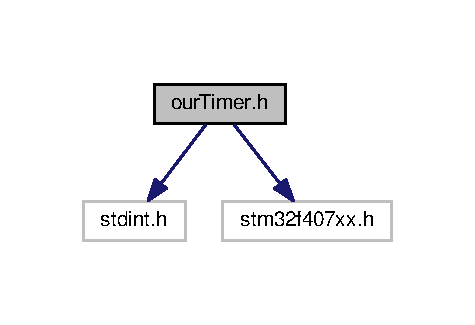
\includegraphics[width=228pt]{our_timer_8h__incl}
\end{center}
\end{figure}
This graph shows which files directly or indirectly include this file\+:
\nopagebreak
\begin{figure}[H]
\begin{center}
\leavevmode
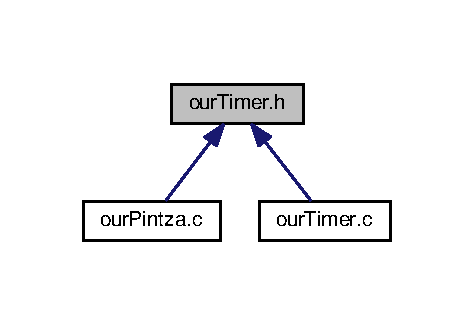
\includegraphics[width=228pt]{our_timer_8h__dep__incl}
\end{center}
\end{figure}
\subsection*{Functions}
\begin{DoxyCompactItemize}
\item 
void \hyperlink{our_timer_8h_a4e742ad28873317354eb02338622cda4}{init\+Timer2} (uint32\+\_\+t ms, uint32\+\_\+t tr\+Go, uint32\+\_\+t interrupzioa)
\item 
void \hyperlink{our_timer_8h_aa7583a2b51bed765f33770ad8ec8b50e}{switch\+Timer2} (int piztu)
\item 
void \hyperlink{our_timer_8h_a984c824e117d7db294dc91fda4bb44f5}{wait\+Tick} (void)
\item 
uint32\+\_\+t \hyperlink{our_timer_8h_a4ac70252749c1e2a3006e0a76b5b9c6e}{get\+Ticks} (void)
\item 
void \hyperlink{our_timer_8h_a4d6ee62b5f61c89897eed1052296d104}{our\+Timer2\+Handler} (void)
\item 
void \hyperlink{our_timer_8h_a4b2ea4175a8cd1eb4d6934a46a69743f}{set\+Timer2\+Call\+Back} (void($\ast$funtzioa)(void))
\end{DoxyCompactItemize}


\subsection{Function Documentation}
\index{our\+Timer.\+h@{our\+Timer.\+h}!get\+Ticks@{get\+Ticks}}
\index{get\+Ticks@{get\+Ticks}!our\+Timer.\+h@{our\+Timer.\+h}}
\subsubsection[{\texorpdfstring{get\+Ticks(void)}{getTicks(void)}}]{\setlength{\rightskip}{0pt plus 5cm}uint32\+\_\+t get\+Ticks (
\begin{DoxyParamCaption}
\item[{void}]{}
\end{DoxyParamCaption}
)}\hypertarget{our_timer_8h_a4ac70252749c1e2a3006e0a76b5b9c6e}{}\label{our_timer_8h_a4ac70252749c1e2a3006e0a76b5b9c6e}
\index{our\+Timer.\+h@{our\+Timer.\+h}!init\+Timer2@{init\+Timer2}}
\index{init\+Timer2@{init\+Timer2}!our\+Timer.\+h@{our\+Timer.\+h}}
\subsubsection[{\texorpdfstring{init\+Timer2(uint32\+\_\+t ms, uint32\+\_\+t tr\+Go, uint32\+\_\+t interrupzioa)}{initTimer2(uint32_t ms, uint32_t trGo, uint32_t interrupzioa)}}]{\setlength{\rightskip}{0pt plus 5cm}void init\+Timer2 (
\begin{DoxyParamCaption}
\item[{uint32\+\_\+t}]{ms, }
\item[{uint32\+\_\+t}]{tr\+Go, }
\item[{uint32\+\_\+t}]{interrupzioa}
\end{DoxyParamCaption}
)}\hypertarget{our_timer_8h_a4e742ad28873317354eb02338622cda4}{}\label{our_timer_8h_a4e742ad28873317354eb02338622cda4}
Initializes timer 2 setting basic configurations for launch. Some given paramaters such as tr\+Go and interrupzio are optional. 
\begin{DoxyParams}{Parameters}
{\em ms} & uint32\+\_\+t type time in millisecond above which timer 2 have to operate. \\
\hline
{\em tr\+Go} & uint32\+\_\+t acts as boolean to know whether is needed to enable T\+R\+GO signal. \\
\hline
{\em interrupzioa} & uint32\+\_\+t acts as a boolean to know whether interruption configuration is needed. \\
\hline
\end{DoxyParams}
\begin{DoxyReturn}{Returns}
void. 
\end{DoxyReturn}
\index{our\+Timer.\+h@{our\+Timer.\+h}!our\+Timer2\+Handler@{our\+Timer2\+Handler}}
\index{our\+Timer2\+Handler@{our\+Timer2\+Handler}!our\+Timer.\+h@{our\+Timer.\+h}}
\subsubsection[{\texorpdfstring{our\+Timer2\+Handler(void)}{ourTimer2Handler(void)}}]{\setlength{\rightskip}{0pt plus 5cm}void our\+Timer2\+Handler (
\begin{DoxyParamCaption}
\item[{void}]{}
\end{DoxyParamCaption}
)}\hypertarget{our_timer_8h_a4d6ee62b5f61c89897eed1052296d104}{}\label{our_timer_8h_a4d6ee62b5f61c89897eed1052296d104}
Custom handler for Timer 2 interruption. \begin{DoxyReturn}{Returns}
void. 
\end{DoxyReturn}
\index{our\+Timer.\+h@{our\+Timer.\+h}!set\+Timer2\+Call\+Back@{set\+Timer2\+Call\+Back}}
\index{set\+Timer2\+Call\+Back@{set\+Timer2\+Call\+Back}!our\+Timer.\+h@{our\+Timer.\+h}}
\subsubsection[{\texorpdfstring{set\+Timer2\+Call\+Back(void($\ast$funtzioa)(void))}{setTimer2CallBack(void(*funtzioa)(void))}}]{\setlength{\rightskip}{0pt plus 5cm}void set\+Timer2\+Call\+Back (
\begin{DoxyParamCaption}
\item[{void($\ast$)(void)}]{funtzioa}
\end{DoxyParamCaption}
)}\hypertarget{our_timer_8h_a4b2ea4175a8cd1eb4d6934a46a69743f}{}\label{our_timer_8h_a4b2ea4175a8cd1eb4d6934a46a69743f}
\index{our\+Timer.\+h@{our\+Timer.\+h}!switch\+Timer2@{switch\+Timer2}}
\index{switch\+Timer2@{switch\+Timer2}!our\+Timer.\+h@{our\+Timer.\+h}}
\subsubsection[{\texorpdfstring{switch\+Timer2(int piztu)}{switchTimer2(int piztu)}}]{\setlength{\rightskip}{0pt plus 5cm}void switch\+Timer2 (
\begin{DoxyParamCaption}
\item[{int}]{piztu}
\end{DoxyParamCaption}
)}\hypertarget{our_timer_8h_aa7583a2b51bed765f33770ad8ec8b50e}{}\label{our_timer_8h_aa7583a2b51bed765f33770ad8ec8b50e}
Enables or disables the Timer 2 depending on the given parameter. 
\begin{DoxyParams}{Parameters}
{\em piztu} & uint32\+\_\+t type acts as a boolean to enable or disable the Timer 2. \\
\hline
\end{DoxyParams}
\begin{DoxyReturn}{Returns}
void. 
\end{DoxyReturn}
\index{our\+Timer.\+h@{our\+Timer.\+h}!wait\+Tick@{wait\+Tick}}
\index{wait\+Tick@{wait\+Tick}!our\+Timer.\+h@{our\+Timer.\+h}}
\subsubsection[{\texorpdfstring{wait\+Tick(void)}{waitTick(void)}}]{\setlength{\rightskip}{0pt plus 5cm}void wait\+Tick (
\begin{DoxyParamCaption}
\item[{void}]{}
\end{DoxyParamCaption}
)}\hypertarget{our_timer_8h_a984c824e117d7db294dc91fda4bb44f5}{}\label{our_timer_8h_a984c824e117d7db294dc91fda4bb44f5}

\hypertarget{our_usart_8c}{}\section{our\+Usart.\+c File Reference}
\label{our_usart_8c}\index{our\+Usart.\+c@{our\+Usart.\+c}}
{\ttfamily \#include \char`\"{}our\+Usart.\+h\char`\"{}}\\*
{\ttfamily \#include \char`\"{}our\+Rcc\+Gpio.\+h\char`\"{}}\\*
Include dependency graph for our\+Usart.\+c\+:
\nopagebreak
\begin{figure}[H]
\begin{center}
\leavevmode
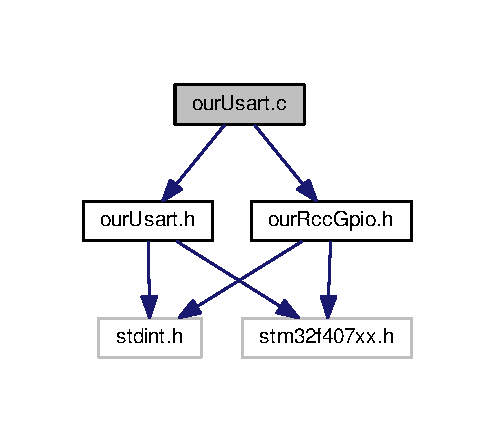
\includegraphics[width=238pt]{our_usart_8c__incl}
\end{center}
\end{figure}
\subsection*{Data Structures}
\begin{DoxyCompactItemize}
\item 
struct \hyperlink{struct_buffer}{Buffer}
\end{DoxyCompactItemize}
\subsection*{Macros}
\begin{DoxyCompactItemize}
\item 
\#define \hyperlink{our_usart_8c_a88e90fe8e8e671220793712eda23c4ab}{U\+S\+A\+R\+T3\+\_\+\+TX}~8
\item 
\#define \hyperlink{our_usart_8c_a240ea511191839f1d66c9d322ad32795}{U\+S\+A\+R\+T3\+\_\+\+RX}~9
\item 
\#define \hyperlink{our_usart_8c_a6b20d41d6252e9871430c242cb1a56e7}{B\+U\+F\+F\+E\+R\+\_\+\+S\+I\+ZE}~20
\end{DoxyCompactItemize}
\subsection*{Typedefs}
\begin{DoxyCompactItemize}
\item 
typedef struct \hyperlink{struct_buffer}{Buffer} \hyperlink{our_usart_8c_a7feadaf37f40473cfc76921f8754c0f7}{Buffer}
\end{DoxyCompactItemize}
\subsection*{Functions}
\begin{DoxyCompactItemize}
\item 
void \hyperlink{our_usart_8c_a80fef8a554a2d8a7293117a350c6d469}{init\+G\+P\+I\+O\+Usart3} (void)
\item 
void \hyperlink{our_usart_8c_a572ec5cdf18960c6e1ca8586d1753cad}{push\+Buffer} (\hyperlink{struct_buffer}{Buffer} $\ast$buffer, uint8\+\_\+t balioa)
\item 
uint8\+\_\+t \hyperlink{our_usart_8c_a04a7f67694cd8c8e656a1a7d52ff4e92}{pop\+Buffer} (\hyperlink{struct_buffer}{Buffer} $\ast$buffer)
\item 
uint32\+\_\+t \hyperlink{our_usart_8c_acf717b26c91cb8efd6cb2fc539ff4a13}{read\+Buffer\+Size} ()
\item 
void \hyperlink{our_usart_8c_a8eefaab45f6957910461f0aed333ab2c}{init\+Usart3} (uint32\+\_\+t baud\+Rate, uint32\+\_\+t interrupzioak)
\item 
void \hyperlink{our_usart_8c_ab022f541e60a58ae01a8187332844406}{write\+Uart3\+Blocking} (uint8\+\_\+t $\ast$mezua, uint32\+\_\+t luzera)
\item 
void \hyperlink{our_usart_8c_adb51cfeefed512873e010a057ccb3c22}{write\+Byte} (uint8\+\_\+t mezua)
\item 
void \hyperlink{our_usart_8c_a243850802a547d297effa71eb4ea52aa}{write\+Uart3} (uint8\+\_\+t $\ast$mezua, uint32\+\_\+t luzera)
\item 
uint32\+\_\+t \hyperlink{our_usart_8c_a4f068b8be3856907f280f139907a25c3}{read\+Uart3} (uint8\+\_\+t $\ast$p\+Msg, uint32\+\_\+t max\+Len)
\item 
void \hyperlink{our_usart_8c_a24944fb8ee8f758c72f61131e65de9ea}{our\+U\+S\+A\+R\+T3\+Handler} ()
\end{DoxyCompactItemize}
\subsection*{Variables}
\begin{DoxyCompactItemize}
\item 
\hyperlink{struct_buffer}{Buffer} \hyperlink{our_usart_8c_ad319ba2f424c53dc8f1a72997d23e010}{buffer\+Idatzi}
\item 
\hyperlink{struct_buffer}{Buffer} \hyperlink{our_usart_8c_a4c7600ddf316259dd8264bc2ae671332}{buffer\+Irakurri}
\end{DoxyCompactItemize}


\subsection{Macro Definition Documentation}
\index{our\+Usart.\+c@{our\+Usart.\+c}!B\+U\+F\+F\+E\+R\+\_\+\+S\+I\+ZE@{B\+U\+F\+F\+E\+R\+\_\+\+S\+I\+ZE}}
\index{B\+U\+F\+F\+E\+R\+\_\+\+S\+I\+ZE@{B\+U\+F\+F\+E\+R\+\_\+\+S\+I\+ZE}!our\+Usart.\+c@{our\+Usart.\+c}}
\subsubsection[{\texorpdfstring{B\+U\+F\+F\+E\+R\+\_\+\+S\+I\+ZE}{BUFFER_SIZE}}]{\setlength{\rightskip}{0pt plus 5cm}\#define B\+U\+F\+F\+E\+R\+\_\+\+S\+I\+ZE~20}\hypertarget{our_usart_8c_a6b20d41d6252e9871430c242cb1a56e7}{}\label{our_usart_8c_a6b20d41d6252e9871430c242cb1a56e7}
\index{our\+Usart.\+c@{our\+Usart.\+c}!U\+S\+A\+R\+T3\+\_\+\+RX@{U\+S\+A\+R\+T3\+\_\+\+RX}}
\index{U\+S\+A\+R\+T3\+\_\+\+RX@{U\+S\+A\+R\+T3\+\_\+\+RX}!our\+Usart.\+c@{our\+Usart.\+c}}
\subsubsection[{\texorpdfstring{U\+S\+A\+R\+T3\+\_\+\+RX}{USART3_RX}}]{\setlength{\rightskip}{0pt plus 5cm}\#define U\+S\+A\+R\+T3\+\_\+\+RX~9}\hypertarget{our_usart_8c_a240ea511191839f1d66c9d322ad32795}{}\label{our_usart_8c_a240ea511191839f1d66c9d322ad32795}
\index{our\+Usart.\+c@{our\+Usart.\+c}!U\+S\+A\+R\+T3\+\_\+\+TX@{U\+S\+A\+R\+T3\+\_\+\+TX}}
\index{U\+S\+A\+R\+T3\+\_\+\+TX@{U\+S\+A\+R\+T3\+\_\+\+TX}!our\+Usart.\+c@{our\+Usart.\+c}}
\subsubsection[{\texorpdfstring{U\+S\+A\+R\+T3\+\_\+\+TX}{USART3_TX}}]{\setlength{\rightskip}{0pt plus 5cm}\#define U\+S\+A\+R\+T3\+\_\+\+TX~8}\hypertarget{our_usart_8c_a88e90fe8e8e671220793712eda23c4ab}{}\label{our_usart_8c_a88e90fe8e8e671220793712eda23c4ab}


\subsection{Typedef Documentation}
\index{our\+Usart.\+c@{our\+Usart.\+c}!Buffer@{Buffer}}
\index{Buffer@{Buffer}!our\+Usart.\+c@{our\+Usart.\+c}}
\subsubsection[{\texorpdfstring{Buffer}{Buffer}}]{\setlength{\rightskip}{0pt plus 5cm}typedef struct {\bf Buffer} {\bf Buffer}}\hypertarget{our_usart_8c_a7feadaf37f40473cfc76921f8754c0f7}{}\label{our_usart_8c_a7feadaf37f40473cfc76921f8754c0f7}


\subsection{Function Documentation}
\index{our\+Usart.\+c@{our\+Usart.\+c}!init\+G\+P\+I\+O\+Usart3@{init\+G\+P\+I\+O\+Usart3}}
\index{init\+G\+P\+I\+O\+Usart3@{init\+G\+P\+I\+O\+Usart3}!our\+Usart.\+c@{our\+Usart.\+c}}
\subsubsection[{\texorpdfstring{init\+G\+P\+I\+O\+Usart3(void)}{initGPIOUsart3(void)}}]{\setlength{\rightskip}{0pt plus 5cm}void init\+G\+P\+I\+O\+Usart3 (
\begin{DoxyParamCaption}
{}
\end{DoxyParamCaption}
)}\hypertarget{our_usart_8c_a80fef8a554a2d8a7293117a350c6d469}{}\label{our_usart_8c_a80fef8a554a2d8a7293117a350c6d469}
Launchs the G\+P\+IO ports needed by Usart to work. \begin{DoxyReturn}{Returns}
void. 
\end{DoxyReturn}
\index{our\+Usart.\+c@{our\+Usart.\+c}!init\+Usart3@{init\+Usart3}}
\index{init\+Usart3@{init\+Usart3}!our\+Usart.\+c@{our\+Usart.\+c}}
\subsubsection[{\texorpdfstring{init\+Usart3(uint32\+\_\+t baud\+Rate, uint32\+\_\+t interrupzioak)}{initUsart3(uint32_t baudRate, uint32_t interrupzioak)}}]{\setlength{\rightskip}{0pt plus 5cm}void init\+Usart3 (
\begin{DoxyParamCaption}
\item[{uint32\+\_\+t}]{baud\+Rate, }
\item[{uint32\+\_\+t}]{interrupzioak}
\end{DoxyParamCaption}
)}\hypertarget{our_usart_8c_a8eefaab45f6957910461f0aed333ab2c}{}\label{our_usart_8c_a8eefaab45f6957910461f0aed333ab2c}
Initializes Usart 3 with a given baudrate and optional configuration for interruption. 
\begin{DoxyParams}{Parameters}
{\em baudrate} & uint32\+\_\+t type specifies the baudrate of Usart.  interrupzioak\+: uint32\+\_\+t acts as a boolean to define whether is needed interrupion configuration. \\
\hline
\end{DoxyParams}
\begin{DoxyReturn}{Returns}
void. 
\end{DoxyReturn}
\index{our\+Usart.\+c@{our\+Usart.\+c}!our\+U\+S\+A\+R\+T3\+Handler@{our\+U\+S\+A\+R\+T3\+Handler}}
\index{our\+U\+S\+A\+R\+T3\+Handler@{our\+U\+S\+A\+R\+T3\+Handler}!our\+Usart.\+c@{our\+Usart.\+c}}
\subsubsection[{\texorpdfstring{our\+U\+S\+A\+R\+T3\+Handler()}{ourUSART3Handler()}}]{\setlength{\rightskip}{0pt plus 5cm}void our\+U\+S\+A\+R\+T3\+Handler (
\begin{DoxyParamCaption}
\item[{void}]{}
\end{DoxyParamCaption}
)}\hypertarget{our_usart_8c_a24944fb8ee8f758c72f61131e65de9ea}{}\label{our_usart_8c_a24944fb8ee8f758c72f61131e65de9ea}
\index{our\+Usart.\+c@{our\+Usart.\+c}!pop\+Buffer@{pop\+Buffer}}
\index{pop\+Buffer@{pop\+Buffer}!our\+Usart.\+c@{our\+Usart.\+c}}
\subsubsection[{\texorpdfstring{pop\+Buffer(\+Buffer $\ast$buffer)}{popBuffer(Buffer *buffer)}}]{\setlength{\rightskip}{0pt plus 5cm}uint8\+\_\+t pop\+Buffer (
\begin{DoxyParamCaption}
\item[{{\bf Buffer} $\ast$}]{buffer}
\end{DoxyParamCaption}
)}\hypertarget{our_usart_8c_a04a7f67694cd8c8e656a1a7d52ff4e92}{}\label{our_usart_8c_a04a7f67694cd8c8e656a1a7d52ff4e92}
Pops the first value of the given buffer. 
\begin{DoxyParams}{Parameters}
{\em buffer} & \hyperlink{struct_buffer}{Buffer} pointer type. \\
\hline
\end{DoxyParams}
\begin{DoxyReturn}{Returns}
pop\+: the first value of the buffer. 
\end{DoxyReturn}
\index{our\+Usart.\+c@{our\+Usart.\+c}!push\+Buffer@{push\+Buffer}}
\index{push\+Buffer@{push\+Buffer}!our\+Usart.\+c@{our\+Usart.\+c}}
\subsubsection[{\texorpdfstring{push\+Buffer(\+Buffer $\ast$buffer, uint8\+\_\+t balioa)}{pushBuffer(Buffer *buffer, uint8_t balioa)}}]{\setlength{\rightskip}{0pt plus 5cm}void push\+Buffer (
\begin{DoxyParamCaption}
\item[{{\bf Buffer} $\ast$}]{buffer, }
\item[{uint8\+\_\+t}]{balioa}
\end{DoxyParamCaption}
)}\hypertarget{our_usart_8c_a572ec5cdf18960c6e1ca8586d1753cad}{}\label{our_usart_8c_a572ec5cdf18960c6e1ca8586d1753cad}
Pushes a new value to the buffer array. 
\begin{DoxyParams}{Parameters}
{\em buffer} & \hyperlink{struct_buffer}{Buffer} pointer type. \\
\hline
{\em balioa} & uint8\+\_\+t type the value that needs to be pushed into the array \\
\hline
\end{DoxyParams}
\index{our\+Usart.\+c@{our\+Usart.\+c}!read\+Buffer\+Size@{read\+Buffer\+Size}}
\index{read\+Buffer\+Size@{read\+Buffer\+Size}!our\+Usart.\+c@{our\+Usart.\+c}}
\subsubsection[{\texorpdfstring{read\+Buffer\+Size()}{readBufferSize()}}]{\setlength{\rightskip}{0pt plus 5cm}uint32\+\_\+t read\+Buffer\+Size (
\begin{DoxyParamCaption}
\item[{void}]{}
\end{DoxyParamCaption}
)}\hypertarget{our_usart_8c_acf717b26c91cb8efd6cb2fc539ff4a13}{}\label{our_usart_8c_acf717b26c91cb8efd6cb2fc539ff4a13}
\index{our\+Usart.\+c@{our\+Usart.\+c}!read\+Uart3@{read\+Uart3}}
\index{read\+Uart3@{read\+Uart3}!our\+Usart.\+c@{our\+Usart.\+c}}
\subsubsection[{\texorpdfstring{read\+Uart3(uint8\+\_\+t $\ast$p\+Msg, uint32\+\_\+t max\+Len)}{readUart3(uint8_t *pMsg, uint32_t maxLen)}}]{\setlength{\rightskip}{0pt plus 5cm}uint32\+\_\+t read\+Uart3 (
\begin{DoxyParamCaption}
\item[{uint8\+\_\+t $\ast$}]{p\+Msg, }
\item[{uint32\+\_\+t}]{max\+Len}
\end{DoxyParamCaption}
)}\hypertarget{our_usart_8c_a4f068b8be3856907f280f139907a25c3}{}\label{our_usart_8c_a4f068b8be3856907f280f139907a25c3}
\index{our\+Usart.\+c@{our\+Usart.\+c}!write\+Byte@{write\+Byte}}
\index{write\+Byte@{write\+Byte}!our\+Usart.\+c@{our\+Usart.\+c}}
\subsubsection[{\texorpdfstring{write\+Byte(uint8\+\_\+t mezua)}{writeByte(uint8_t mezua)}}]{\setlength{\rightskip}{0pt plus 5cm}void write\+Byte (
\begin{DoxyParamCaption}
\item[{uint8\+\_\+t}]{mezua}
\end{DoxyParamCaption}
)}\hypertarget{our_usart_8c_adb51cfeefed512873e010a057ccb3c22}{}\label{our_usart_8c_adb51cfeefed512873e010a057ccb3c22}
Writes one byte on data register (DR)  mezua\+: uint8\+\_\+t the message that needs to be written in the data register. \begin{DoxyReturn}{Returns}
void. 
\end{DoxyReturn}
\index{our\+Usart.\+c@{our\+Usart.\+c}!write\+Uart3@{write\+Uart3}}
\index{write\+Uart3@{write\+Uart3}!our\+Usart.\+c@{our\+Usart.\+c}}
\subsubsection[{\texorpdfstring{write\+Uart3(uint8\+\_\+t $\ast$mezua, uint32\+\_\+t luzera)}{writeUart3(uint8_t *mezua, uint32_t luzera)}}]{\setlength{\rightskip}{0pt plus 5cm}void write\+Uart3 (
\begin{DoxyParamCaption}
\item[{uint8\+\_\+t $\ast$}]{mezua, }
\item[{uint32\+\_\+t}]{luzera}
\end{DoxyParamCaption}
)}\hypertarget{our_usart_8c_a243850802a547d297effa71eb4ea52aa}{}\label{our_usart_8c_a243850802a547d297effa71eb4ea52aa}
/ Copy the message to the buffer when it can. 
\begin{DoxyParams}{Parameters}
{\em mezua} & uint8\+\_\+t pointer holds the message value. \\
\hline
{\em luzera} & uint32\+\_\+t type the size of the message. \\
\hline
\end{DoxyParams}
\begin{DoxyReturn}{Returns}
void. 
\end{DoxyReturn}
\index{our\+Usart.\+c@{our\+Usart.\+c}!write\+Uart3\+Blocking@{write\+Uart3\+Blocking}}
\index{write\+Uart3\+Blocking@{write\+Uart3\+Blocking}!our\+Usart.\+c@{our\+Usart.\+c}}
\subsubsection[{\texorpdfstring{write\+Uart3\+Blocking(uint8\+\_\+t $\ast$mezua, uint32\+\_\+t luzera)}{writeUart3Blocking(uint8_t *mezua, uint32_t luzera)}}]{\setlength{\rightskip}{0pt plus 5cm}void write\+Uart3\+Blocking (
\begin{DoxyParamCaption}
\item[{uint8\+\_\+t $\ast$}]{mezua, }
\item[{uint32\+\_\+t}]{luzera}
\end{DoxyParamCaption}
)}\hypertarget{our_usart_8c_ab022f541e60a58ae01a8187332844406}{}\label{our_usart_8c_ab022f541e60a58ae01a8187332844406}


\subsection{Variable Documentation}
\index{our\+Usart.\+c@{our\+Usart.\+c}!buffer\+Idatzi@{buffer\+Idatzi}}
\index{buffer\+Idatzi@{buffer\+Idatzi}!our\+Usart.\+c@{our\+Usart.\+c}}
\subsubsection[{\texorpdfstring{buffer\+Idatzi}{bufferIdatzi}}]{\setlength{\rightskip}{0pt plus 5cm}{\bf Buffer} buffer\+Idatzi}\hypertarget{our_usart_8c_ad319ba2f424c53dc8f1a72997d23e010}{}\label{our_usart_8c_ad319ba2f424c53dc8f1a72997d23e010}
\index{our\+Usart.\+c@{our\+Usart.\+c}!buffer\+Irakurri@{buffer\+Irakurri}}
\index{buffer\+Irakurri@{buffer\+Irakurri}!our\+Usart.\+c@{our\+Usart.\+c}}
\subsubsection[{\texorpdfstring{buffer\+Irakurri}{bufferIrakurri}}]{\setlength{\rightskip}{0pt plus 5cm}{\bf Buffer} buffer\+Irakurri}\hypertarget{our_usart_8c_a4c7600ddf316259dd8264bc2ae671332}{}\label{our_usart_8c_a4c7600ddf316259dd8264bc2ae671332}

\hypertarget{our_usart_8h}{}\section{our\+Usart.\+h File Reference}
\label{our_usart_8h}\index{our\+Usart.\+h@{our\+Usart.\+h}}
{\ttfamily \#include $<$stdint.\+h$>$}\\*
{\ttfamily \#include $<$stm32f407xx.\+h$>$}\\*
Include dependency graph for our\+Usart.\+h\+:
\nopagebreak
\begin{figure}[H]
\begin{center}
\leavevmode
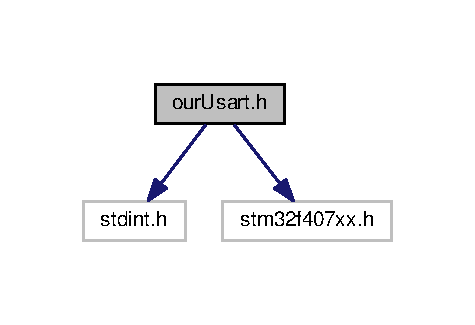
\includegraphics[width=228pt]{our_usart_8h__incl}
\end{center}
\end{figure}
This graph shows which files directly or indirectly include this file\+:
\nopagebreak
\begin{figure}[H]
\begin{center}
\leavevmode
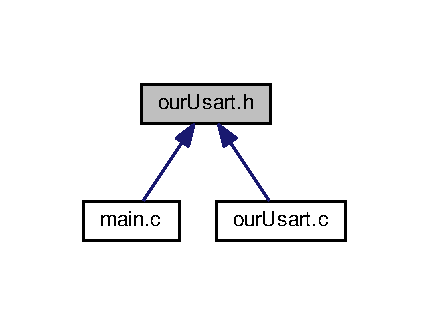
\includegraphics[width=206pt]{our_usart_8h__dep__incl}
\end{center}
\end{figure}
\subsection*{Functions}
\begin{DoxyCompactItemize}
\item 
void \hyperlink{our_usart_8h_a8eefaab45f6957910461f0aed333ab2c}{init\+Usart3} (uint32\+\_\+t baud\+Rate, uint32\+\_\+t interrupzioak)
\item 
uint32\+\_\+t \hyperlink{our_usart_8h_a4794ef7159391d61499e9f16656255e9}{read\+Buffer\+Size} (void)
\item 
void \hyperlink{our_usart_8h_a243850802a547d297effa71eb4ea52aa}{write\+Uart3} (uint8\+\_\+t $\ast$mezua, uint32\+\_\+t luzera)
\item 
uint32\+\_\+t \hyperlink{our_usart_8h_a4f068b8be3856907f280f139907a25c3}{read\+Uart3} (uint8\+\_\+t $\ast$p\+Msg, uint32\+\_\+t max\+Len)
\item 
void \hyperlink{our_usart_8h_ab022f541e60a58ae01a8187332844406}{write\+Uart3\+Blocking} (uint8\+\_\+t $\ast$mezua, uint32\+\_\+t luzera)
\item 
void \hyperlink{our_usart_8h_adb51cfeefed512873e010a057ccb3c22}{write\+Byte} (uint8\+\_\+t mezua)
\item 
void \hyperlink{our_usart_8h_a86527d5272d5802e3ddd5dc520c92083}{our\+U\+S\+A\+R\+T3\+Handler} (void)
\item 
void \hyperlink{our_usart_8h_ac4ade44b3bb844f1d1fc2757451a0008}{write\+To\+Uart} (uint8\+\_\+t $\ast$p\+Msg)
\end{DoxyCompactItemize}


\subsection{Function Documentation}
\index{our\+Usart.\+h@{our\+Usart.\+h}!init\+Usart3@{init\+Usart3}}
\index{init\+Usart3@{init\+Usart3}!our\+Usart.\+h@{our\+Usart.\+h}}
\subsubsection[{\texorpdfstring{init\+Usart3(uint32\+\_\+t baud\+Rate, uint32\+\_\+t interrupzioak)}{initUsart3(uint32_t baudRate, uint32_t interrupzioak)}}]{\setlength{\rightskip}{0pt plus 5cm}void init\+Usart3 (
\begin{DoxyParamCaption}
\item[{uint32\+\_\+t}]{baud\+Rate, }
\item[{uint32\+\_\+t}]{interrupzioak}
\end{DoxyParamCaption}
)}\hypertarget{our_usart_8h_a8eefaab45f6957910461f0aed333ab2c}{}\label{our_usart_8h_a8eefaab45f6957910461f0aed333ab2c}
Initializes Usart 3 with a given baudrate and optional configuration for interruption. 
\begin{DoxyParams}{Parameters}
{\em baudrate} & uint32\+\_\+t type specifies the baudrate of Usart.  interrupzioak\+: uint32\+\_\+t acts as a boolean to define whether is needed interrupion configuration. \\
\hline
\end{DoxyParams}
\begin{DoxyReturn}{Returns}
void. 
\end{DoxyReturn}
\index{our\+Usart.\+h@{our\+Usart.\+h}!our\+U\+S\+A\+R\+T3\+Handler@{our\+U\+S\+A\+R\+T3\+Handler}}
\index{our\+U\+S\+A\+R\+T3\+Handler@{our\+U\+S\+A\+R\+T3\+Handler}!our\+Usart.\+h@{our\+Usart.\+h}}
\subsubsection[{\texorpdfstring{our\+U\+S\+A\+R\+T3\+Handler(void)}{ourUSART3Handler(void)}}]{\setlength{\rightskip}{0pt plus 5cm}void our\+U\+S\+A\+R\+T3\+Handler (
\begin{DoxyParamCaption}
\item[{void}]{}
\end{DoxyParamCaption}
)}\hypertarget{our_usart_8h_a86527d5272d5802e3ddd5dc520c92083}{}\label{our_usart_8h_a86527d5272d5802e3ddd5dc520c92083}
\index{our\+Usart.\+h@{our\+Usart.\+h}!read\+Buffer\+Size@{read\+Buffer\+Size}}
\index{read\+Buffer\+Size@{read\+Buffer\+Size}!our\+Usart.\+h@{our\+Usart.\+h}}
\subsubsection[{\texorpdfstring{read\+Buffer\+Size(void)}{readBufferSize(void)}}]{\setlength{\rightskip}{0pt plus 5cm}uint32\+\_\+t read\+Buffer\+Size (
\begin{DoxyParamCaption}
\item[{void}]{}
\end{DoxyParamCaption}
)}\hypertarget{our_usart_8h_a4794ef7159391d61499e9f16656255e9}{}\label{our_usart_8h_a4794ef7159391d61499e9f16656255e9}
\index{our\+Usart.\+h@{our\+Usart.\+h}!read\+Uart3@{read\+Uart3}}
\index{read\+Uart3@{read\+Uart3}!our\+Usart.\+h@{our\+Usart.\+h}}
\subsubsection[{\texorpdfstring{read\+Uart3(uint8\+\_\+t $\ast$p\+Msg, uint32\+\_\+t max\+Len)}{readUart3(uint8_t *pMsg, uint32_t maxLen)}}]{\setlength{\rightskip}{0pt plus 5cm}uint32\+\_\+t read\+Uart3 (
\begin{DoxyParamCaption}
\item[{uint8\+\_\+t $\ast$}]{p\+Msg, }
\item[{uint32\+\_\+t}]{max\+Len}
\end{DoxyParamCaption}
)}\hypertarget{our_usart_8h_a4f068b8be3856907f280f139907a25c3}{}\label{our_usart_8h_a4f068b8be3856907f280f139907a25c3}
\index{our\+Usart.\+h@{our\+Usart.\+h}!write\+Byte@{write\+Byte}}
\index{write\+Byte@{write\+Byte}!our\+Usart.\+h@{our\+Usart.\+h}}
\subsubsection[{\texorpdfstring{write\+Byte(uint8\+\_\+t mezua)}{writeByte(uint8_t mezua)}}]{\setlength{\rightskip}{0pt plus 5cm}void write\+Byte (
\begin{DoxyParamCaption}
\item[{uint8\+\_\+t}]{mezua}
\end{DoxyParamCaption}
)}\hypertarget{our_usart_8h_adb51cfeefed512873e010a057ccb3c22}{}\label{our_usart_8h_adb51cfeefed512873e010a057ccb3c22}
Writes one byte on data register (DR)  mezua\+: uint8\+\_\+t the message that needs to be written in the data register. \begin{DoxyReturn}{Returns}
void. 
\end{DoxyReturn}
\index{our\+Usart.\+h@{our\+Usart.\+h}!write\+To\+Uart@{write\+To\+Uart}}
\index{write\+To\+Uart@{write\+To\+Uart}!our\+Usart.\+h@{our\+Usart.\+h}}
\subsubsection[{\texorpdfstring{write\+To\+Uart(uint8\+\_\+t $\ast$p\+Msg)}{writeToUart(uint8_t *pMsg)}}]{\setlength{\rightskip}{0pt plus 5cm}void write\+To\+Uart (
\begin{DoxyParamCaption}
\item[{uint8\+\_\+t $\ast$}]{p\+Msg}
\end{DoxyParamCaption}
)}\hypertarget{our_usart_8h_ac4ade44b3bb844f1d1fc2757451a0008}{}\label{our_usart_8h_ac4ade44b3bb844f1d1fc2757451a0008}
\index{our\+Usart.\+h@{our\+Usart.\+h}!write\+Uart3@{write\+Uart3}}
\index{write\+Uart3@{write\+Uart3}!our\+Usart.\+h@{our\+Usart.\+h}}
\subsubsection[{\texorpdfstring{write\+Uart3(uint8\+\_\+t $\ast$mezua, uint32\+\_\+t luzera)}{writeUart3(uint8_t *mezua, uint32_t luzera)}}]{\setlength{\rightskip}{0pt plus 5cm}void write\+Uart3 (
\begin{DoxyParamCaption}
\item[{uint8\+\_\+t $\ast$}]{mezua, }
\item[{uint32\+\_\+t}]{luzera}
\end{DoxyParamCaption}
)}\hypertarget{our_usart_8h_a243850802a547d297effa71eb4ea52aa}{}\label{our_usart_8h_a243850802a547d297effa71eb4ea52aa}
/ Copy the message to the buffer when it can. 
\begin{DoxyParams}{Parameters}
{\em mezua} & uint8\+\_\+t pointer holds the message value. \\
\hline
{\em luzera} & uint32\+\_\+t type the size of the message. \\
\hline
\end{DoxyParams}
\begin{DoxyReturn}{Returns}
void. 
\end{DoxyReturn}
\index{our\+Usart.\+h@{our\+Usart.\+h}!write\+Uart3\+Blocking@{write\+Uart3\+Blocking}}
\index{write\+Uart3\+Blocking@{write\+Uart3\+Blocking}!our\+Usart.\+h@{our\+Usart.\+h}}
\subsubsection[{\texorpdfstring{write\+Uart3\+Blocking(uint8\+\_\+t $\ast$mezua, uint32\+\_\+t luzera)}{writeUart3Blocking(uint8_t *mezua, uint32_t luzera)}}]{\setlength{\rightskip}{0pt plus 5cm}void write\+Uart3\+Blocking (
\begin{DoxyParamCaption}
\item[{uint8\+\_\+t $\ast$}]{mezua, }
\item[{uint32\+\_\+t}]{luzera}
\end{DoxyParamCaption}
)}\hypertarget{our_usart_8h_ab022f541e60a58ae01a8187332844406}{}\label{our_usart_8h_ab022f541e60a58ae01a8187332844406}

%--- End generated contents ---

% Index
\backmatter
\newpage
\phantomsection
\clearemptydoublepage
\addcontentsline{toc}{chapter}{Index}
\printindex

\end{document}
